
\part{The Fundamentals of Diabetes}

\newpage
~\phantom{a}
\thispagestyle{empty}
\newpage


\chapter{The history of diabetes}\label{chap1}

\textbf{Diabetes\index{Diabetes}—historical background and milestones}

When one looks back at the history of diabetes, several\break strange facts emerge. In fact in this day and age, we may even find these beliefs of our ancestors somewhat funny.

\begin{wrapfigure}{l}{5cm}
\vskip -.4cm
\centering
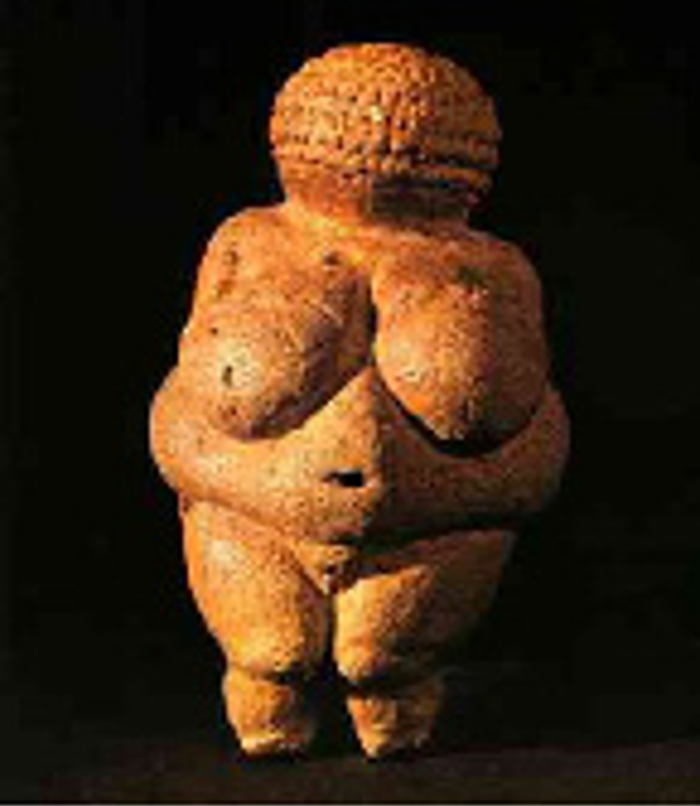
\includegraphics[scale=.9]{images/004.jpg}\\
\textbf{\textit{Venus of Willendorf}}
\vskip -.4cm
\end{wrapfigure}
You would find it amusing to know that overweight people were conside\-red celebrities in ancient times. Civilizations of the Medite\-rranean region (Greeks, Egyptians, Mesopotamians) considered overweight indi\-viduals both wealthy and healthy. They pitied the lean as unfortunate and deprived of health. This belief was so strong as to give rise to sayings such as “stoutness is the sister of beauty”, and “stoutness makes a mare (a female horse) lovely, let alone a maid”.

The people of Austria (in Europe) used to worship ‘Venus of Willendorf’, an 11–cm female statuette with exaggerated breasts, abdomen and pelvis, as the Goddess of fertility. It is obvious from this practice that being fleshy was equated with health and fertility.


With the passage of time, several of these beliefs were proven to be false. In the 4th century B.C., Hippocrates in his ‘Aphorisms’ stated, “Persons who are naturally fat are more apt to die earlier than those who are slender” (Aphorisms II: 44).

\begin{wrapfigure}{l}{4.5cm}
\centering
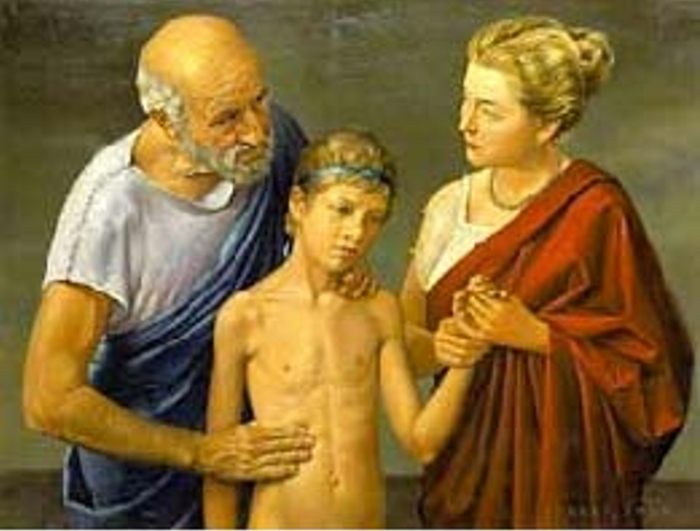
\includegraphics[scale=.9]{images/005.jpg}\\
\textbf{\textit{Hippocrates}}
\vskip -.5cm
\end{wrapfigure}

Hippocrates also described the sy\-mptoms of diabetes in the 4th century B.C. Hippocrates is widely considered as the “father of modern medicine”. He autho\-red the ‘Hippocratic Oath’, the original docu\-ment on the ethics of medical pra\-ctice. Even to this day it serves as a guide to doctors about\break patient etiquette, and also about utilizing medical know\-ledge, skill, and compa\-ssion to serve as a friend, philosopher, and guide in the\break society.

\begin{wrapfigure}{l}{4cm}
\centering
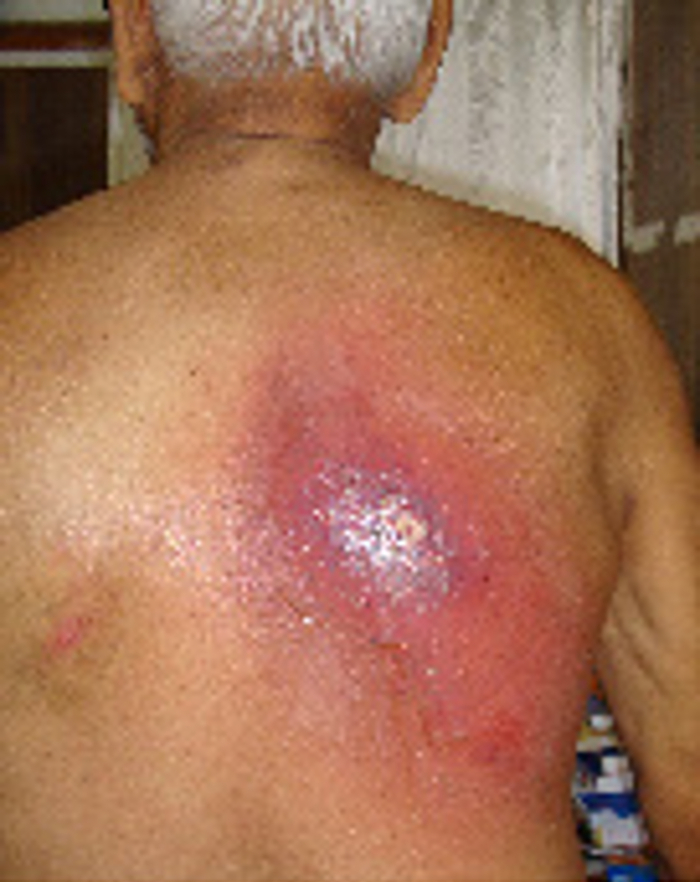
\includegraphics[scale=.7]{images/006.jpg}\\
\textbf{\textit{Carbuncle}}
\vskip -.4cm
\end{wrapfigure}

Diabetes is not a new disease. It dates back to the origins of humankind itself. In fact, if we flip through the pages of\break history in our own country, there are\break several refe\-rences to this disease. In Te\-lugu folklore, one of the manifestations of this disease was termed \textit{“raasapundu”} (royal abscess) or an abscess (a collection of pus) that deve\-loped among royal\break families. This has been described in detail in the story of the King of Kambhoj. This abscess was usually seen on the nape of the neck and the back, and is now termed a  ‘carbu\-ncle’. A carbuncle is a pus collection that is larger than a boil, and it tends to drain pus through multiple openings.\break Carbuncles or abscesses are commonly seen skin infections in diabetes. Since there were no medicines to treat these pus collections in the\break ancient times, they would fester for prolonged periods of time. Since this condition was seen only among the wealthy at that time, this was called a “royal wound or abscess”.

‘\textit{Charaka Samhita}’ and ‘\textit{Sushrutha Samhita}’ are two ancient\break Indian treatises of Ayurveda. \textit{Charaka Samhita} describes four\break cardinal principles of preventive medicine, namely:

\begin{enumerate}
\itemsep=0pt
\item ‘\textit{Aachara}’ or how we conduct ourselves
\item ‘\textit{Aahara}’ or food habits
\item ‘\textit{Vyaayama}’ or physical exercise
\item ‘\textit{Yoga}’ or mental balance to stabilize the mind and body.
\end{enumerate}

\vskip -.2cm
These simple principles recommended by Charaka almost\break 2300 years ago, seem all the more relevant in the present time to\break prevent the uncontrolled growth of diabetes.

The Egyptians have described the history of diabetes, and signs and symptoms of the disease in medical books dating back to 1552.

Several great personalities have recorded their experiences with diabetes since the ancient ages to the present day.

In 1674, Thomas Willis officially coined the term “Diabetes\break Mellitus”. Thomas Willis was a pioneer researcher of the ana\-tomy of the brain and nervous system. He is credited with disco\-vering a part of the brain now known as the “circle of Willis”. He documented that urine of patients with diabetes is sweet.

However, the great Sushrutha had observed this much\break earlier, and had coined the term \textit{“madhumeha”} or “sweet urine\break disease”.

\begin{wrapfigure}{l}{4cm}
\centering
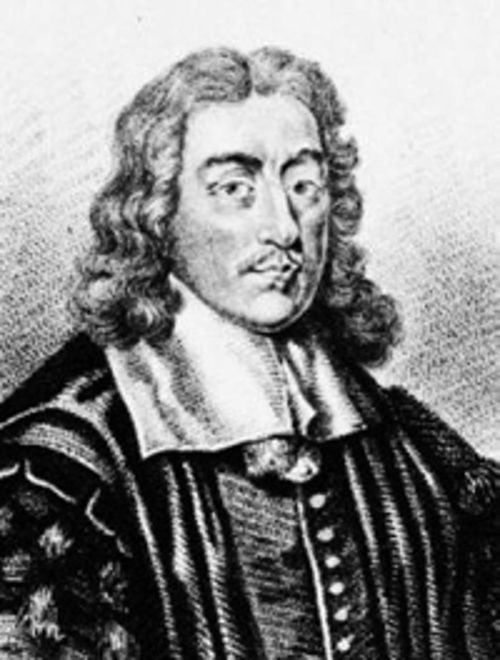
\includegraphics[scale=1]{images/007.jpg}\\
\textbf{\textit{Thomas Willis}}
\vskip -.6cm
\end{wrapfigure}

But Thomas Willis is credited with retesting this theory. He observed that ants made a beeline to a diabetic’s urine. Since ants are attracted to anything sweet, he hypothesized that the urine must be sweet. The brave soul that he was, he placed a drop of a dia\-betic’s urine on his own tongue, and confirmed that it was\break indeed sweet!

Thomas Willis went on to call this\break disease a “pissing evil”, since it manifests as excess urination, and noted that in patients with diabetes “the urine is wonderfully sweet, as if imbued with honey or sugar”.

In 1776, Mathew Dobson, inspired by Thomas Willis’s scientific\break theories came up with experimental evidence confirming the presence of sugar in a diabetic’s urine. He gently heated a dia\-betic’s urine till\break all the liquid evaporated. He was left with a whitish residue, which\break was nothing but sugar$^{\text{\cite{chap1–key01}}}$. This explained the sweetness of urine.\break Dobson detailed his findings in a paper presented to the Medical\break Society of London.


With this background, let us explore the origin of the word\break “diabetes mellitus”. Diabetes in Greek means “pass through a tube”. Mellitus is the Latin word for honey. Since excess sweet urine passes through the urethra (tube through which urine is excreted from the body), the term “Diabetes Mellitus” was coined.

In Sanskrit, \textit{“madhu’} means honey, and \textit{“meha”} means urine, thus \textit{“madhumeha”} is the exact equivalent for ‘diabetes mellitus’.

In 1870, Claude Bernard, through his experiments discovered that people suffe\-ring from diabetes had increased produ\-ction of glucose in their bodies. So at this point in history, two principles were scienti\-fically established. First, urine of diabetics contains sugar. And second, there is excess glucose production in dia\-betics.

\begin{wrapfigure}{l}{4cm}
\centering
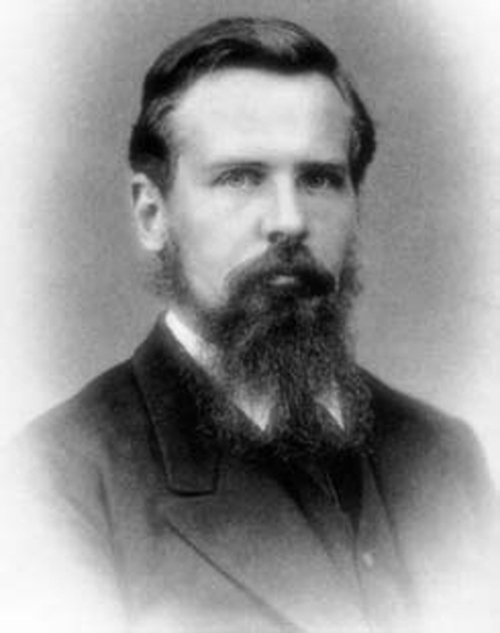
\includegraphics[scale=1]{images/008.jpg}\\
\textbf{\textit{Paul Langerhans}}
\vskip -.5cm
\end{wrapfigure}

The history of diabetes is full of thrilling accounts of medical stude\-nts and doctors playing the role of scientist–investigators to unravel the disease plot!


In 1869, Paul Langerhans, as part of his undergraduate medical\- training at the University of Berlin is credited with the first meticulous description of the microscopic structure of the pancreas in his\break doctoral dissertation. He described nine different types of cells, one of which tended to aggregate together in the form of ‘islands’ throughout the pancreas. It was subsequently discovered that these islands produced insulin. These cell clusters were later named “islets of Langerhans” in his honor.

\begin{wrapfigure}{r}{4.5cm}
\centering
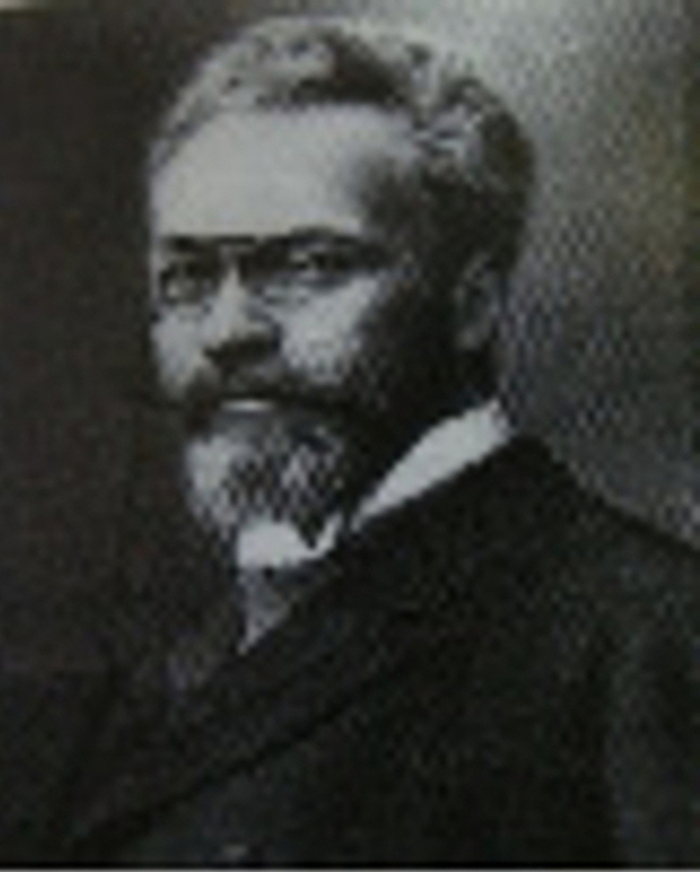
\includegraphics[scale=.8]{images/009.jpg}\\
\textbf{\textit{Oskar Minkowski}}
\vskip -.4cm
\end{wrapfigure}

In 1889, Oskar Minkowski performed a landmark study. He demon\-strated that when the pancreas gland was surgically removed from dogs, they developed diabetes. He thus proved that the pancreas gland is integral to having normal glucose metabolism.

He also went on to describe the\break disease features of diabetes, and noted that people with diabetes wither away because the body literally melts and flows out through their urine.

\begin{wrapfigure}{l}{4.6cm}
\centering
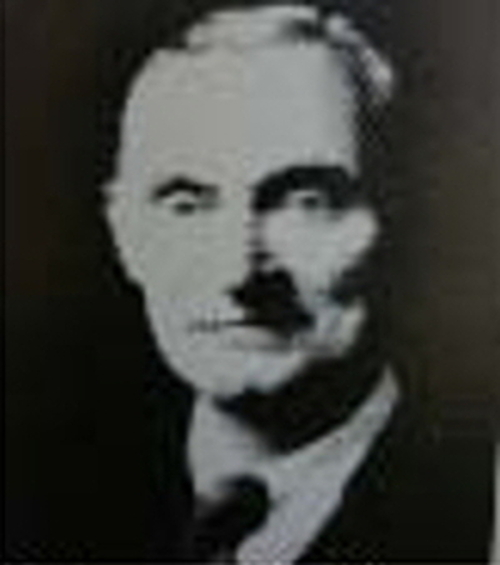
\includegraphics[scale=1.2]{images/010.jpg}\\
\textbf{\textit{Eugene Opie}}
\vskip -.4cm
\end{wrapfigure}

As more studies started to un\-cover many of the mysteries surrou\-nding\break diabetes, investigations into the associ\-ation between the pancreas and dia\-betes were being undertaken. In 1908, Oscar Minkow\-ski in collabo\-ration with Eugene Opie collected the pancrea\-tic extract, and attempted to utilize the active ingredient of this pancreatic\break extract (which we now know to be insu\-lin), in controlling diabetes. Wor\-king on the same principle, in 1908, George Ludwig Zulzer, who was fresh out of medical training and was working as a ‘House Surgeon’ in Berlin, named the hormone found in pancreatic extract ‘acomatrol’. He inje\-cted this extract into five diabetic patients and was successful in controlling the excess sugar\break content in the blood. But due to the impurities found in acomatrol\break extracted from the pancreas gland of a calf, the patients experienced side effects, and died once the supply of acomatrol was exhausted. Sadly, his laboratory was taken over by the German military du\-ring World War I, interrupting his important work. Despite this, George Ludwig, aided by his courage and conviction, scientifically demonstrated two important principles:

\begin{enumerate}
\itemsep=0pt
\item Pancreatic extract contained a substance that could bring down sugar levels in the blood.
\item Pancreatic extract contained impurities, which were an impediment to its safe use in patients with diabetes.
\end{enumerate}

\vskip -.3cm

George Ludwig’s discoveries laid the foundation for work on\break purification of pancreatic extract for human use in the coming years and decades.

In 1909, Jean de Meyer, a Belgian, proposed the name “Insulin” for this glucose lowering hormone in pancreatic extract, derived from the Latin word ‘insula’ meaning island, referring to the islets (or islands) of Langerhans, from where this hormone is produced.

In the early 20th century, in the midst of these developments, a new issue arose. While it is true that there is sugar in the urine of diabetics, how can we objectively demonstrate this? Because doing so may help in establishing the diagnosis of diabetes. Unlike Thomas Willis, it is unlikely that most people would find the idea of confirming the presence of sugar by actually tasting it very ‘palatable’!

In 1911, Stanley Benedict, an American chemist, literally\break came up with the ‘solution’ for this problem. He discovered\break ‘Benedict’s solution or reagent’; a chemical which when added to urine and heated would cause a change in the color of urine, and indicate the presence of sugar! A truly ‘long–lasting solution’ this is, as it has stood the test of time for more than a century and continues to be used in hospitals and laboratories to this day (though newer techniques have emerged over the past half a century).

\begin{center}
\textbf{The team of scientists who discovered Insulin}
\end{center}

{\centering{
\begin{tabular}{@{}cccc@{}}
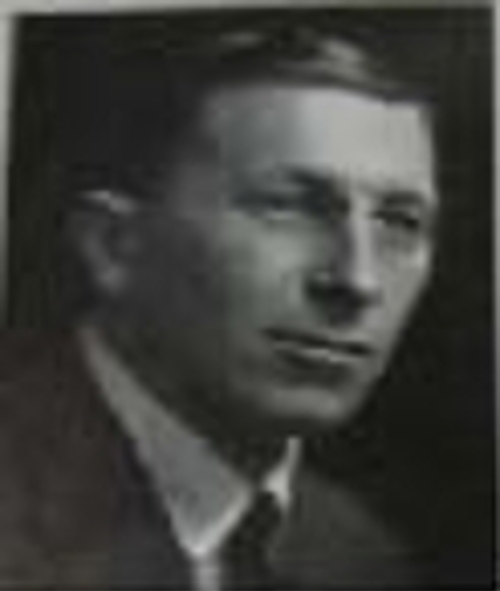
\includegraphics[scale=.55]{images/011.jpg} & 
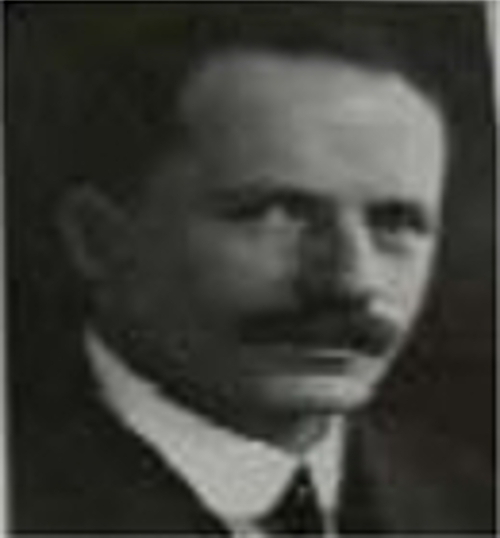
\includegraphics[scale=.6]{images/012.jpg} &
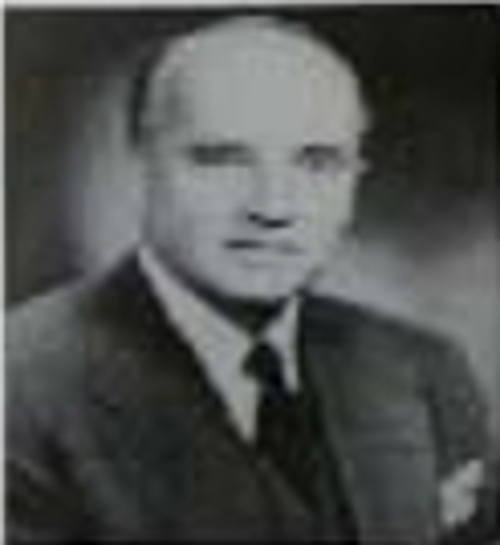
\includegraphics[scale=.6]{images/013.jpg} &
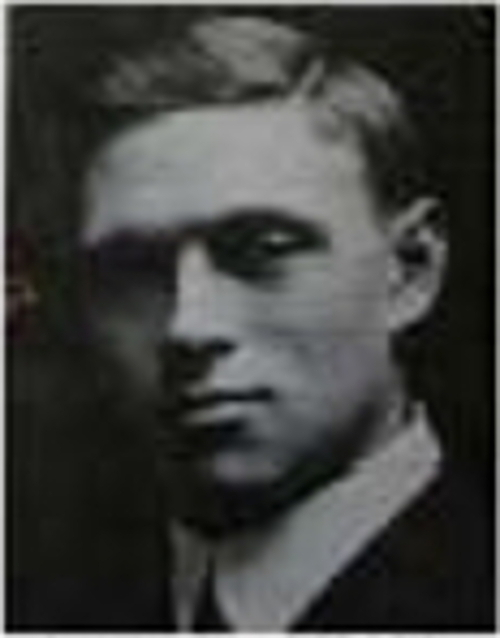
\includegraphics[scale=.5]{images/014.jpg}\\
{\small\textit{\textbf{Frederick Banting}}} &
{\small\textit{\textbf{J.J.R.Macleod}}} &
{\small\textit{\textbf{Charles Herbert Best}}} &
{\small\textit{\textbf{James Collip}}}
\end{tabular}
}}

The years 1921–22 marked a momentous period in the history of diabetes. Frederick Banting, a Canadian doctor and scientist, became deeply interested in diabetes, and began work on trying to isolate insu\-lin from the pancreas in the lab of J.J.R. Macleod, Professor of Physio\-logy at the University of Toronto.

Dr. Charles Herbert Best, a medical student at that time, was\break appointed Banting’s assistant. Later, a young biochemist, James Bert\-ram Collip, was also appointed to assist in this endeavor. This team made one of the greatest discoveries in the history of medicine by\break isolating insulin from the islet cells in the pancreas of dogs. The scienti\-fic world acknowledged their marvelous effort with nothing less than the Nobel Prize in 1923. As of September 2011, Dr. Banting remains the youngest Nobel laureate (at the age of 32) in the area of physio\-logy/medicine.

\begin{wrapfigure}{l}{4cm}
\vskip -.3cm
\centering
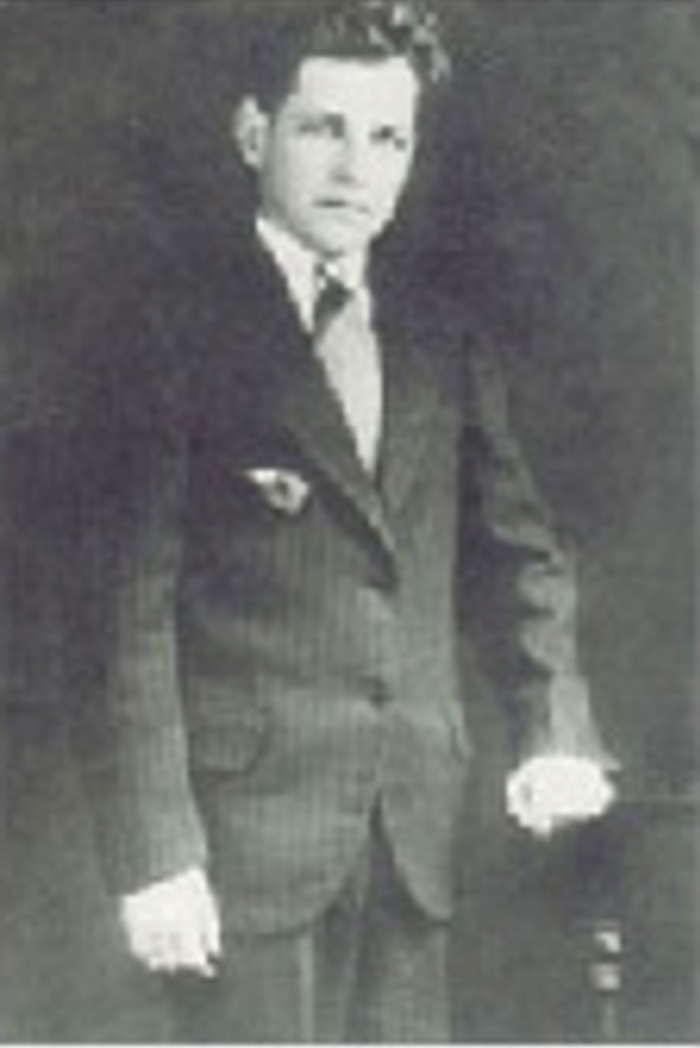
\includegraphics[scale=.7]{images/015.jpg}\\
\textbf{\textit{Leonard Thompson}}
\vskip -.4cm
\end{wrapfigure}

However, as we all know, the proof of the pudding is in the eating. To demonstrate the enormous potential of insulin in treating diabetes, these researchers\break injected insulin into Leonard Thompson, a 14–year–old boy on January 11, 1922. At this time in history, anyone diagnosed with diabetes was resigned to a life of great suffering. The only es\-cape from their\break misery was the inevitable quick death in a matter of days to months. But, in Leonard Thompson’s case, insulin increased his longevity, and he lived for another 13 years. He thus became the first ever patient to be successfully treated for diabetes, and this marked the dawn of a new age in the history of diabetes!

Insulin preparations used in the early days were extracted from canine (dog) and bovine (cow) pancreas. They contained animal proteins in them, and were prone to cause allergic rea\-ctions in patients. Work on purifying insulin in a bid to prevent such allergic reactions continues to this day.

The dramatic isolation of insulin and its introduction into clinical practice seemed to be the ultimate cure for diabetes.

However, in 1936, Sir Harold Himsworth, a graduate of the\break University College Hospital and Medical School, London, proposed an outrageous view in “The Lancet”, a reputed medical journal that not all diabetes is caused by lack of insulin! He introduced the concept of\break ‘insulin sensitivity’. In a series of three lectures at the Royal\break College of Physicians in 1939, he characte\-rized two broad types of\break diabetes. He observed that the diabe\-tics who are sensitive to insulin tend to be younger and thin with normal blood pressure, and usually have a sudden and severe onset of diabetes (now known as Type 1\break diabetes). The diabetics who are insensitive to insulin on the other hand, tend be older, obese, have high blood pressure, and have a more gradual onset of diabetes (now known as Type 2 diabetes).

Coming on the heels of these observations, in 1951, Robert Daniel Lawrence, a British surgeon and a diabetic himself, was able to\break measure the insulin levels in human blood for the first time. He\break measured it in 10 diabetics, and found that young dia\-betics had no\break insulin in their blood, but obese, older diabetics surprisingly showed detectable amounts of insulin in their blood! Interestingly, Robert\break Daniel Lawre\-nce’s vision was impaired significantly due to diabetes\break related eye infections. He got a second lease of life, thanks to the\break discovery of insulin, and dedicated himself to the field of diabetes.

\clearpage

In 1979 the American Diabetic Association recognized these two different forms of diabetes as Type 1 and Type 2 diabetes.

\noindent
\textbf{The discovery of the amino acid sequence of insulin: an\break invaluable contribution to mankind}

The early insulin preparations were hampered by allergic rea\-ctions they elicited in the human body. This was because these insulins were either extracted from the pancreas of cows (bovine insulin) or dogs\break (canine insulin). Thankfully, today we mostly use human insulin,\break which is synthetic insulin less likely to cause allergic reactions. But in order to prepare this synthetic insulin, we need to know the\break ingredients that go into making this insu\-lin. While scientists knew that all proteins are made up of amino acids, up to the 1950s, nobody in the world knew the exact number of amino acids, or the sequence in which they were arranged in an insulin molecule.

\begin{wrapfigure}{l}{4.4cm}
\centering
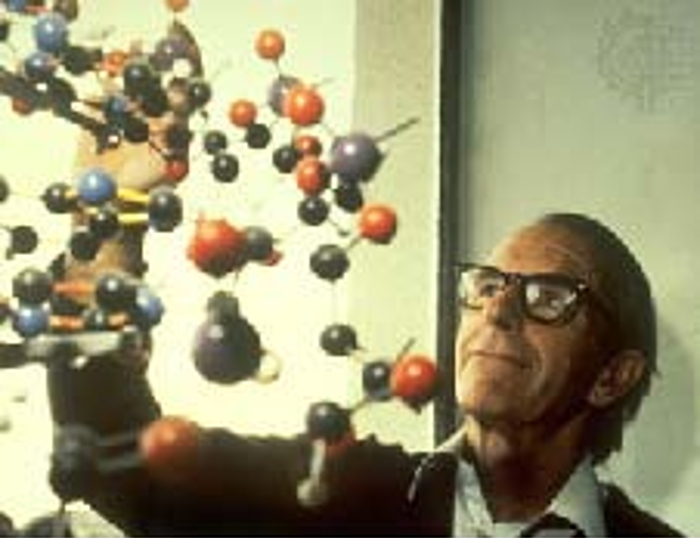
\includegraphics[scale=.9]{images/016.jpg}\\
\textbf{\textit{Fred Sanger (1918–2013) Laconic scientist who decoded the amino acids sequence in insulin}}
\vskip -.3cm
\end{wrapfigure}

Enter Frederick Sanger! In 1943, he set out on an ambitious project to\break decode the biochemical structure of insu\-lin as part of his postdoctoral\break research at the Cambridge University. By 1954, he had not only identified the 51 amino acids that make up the\break insulin molecule, but also the exact\break sequence in which these amino acids were arranged. In this endeavor, he also inve\-nted a way to determine the\break structure of proteins, which could be used to deci\-pher the structure of many proteins other than insulin. For this invaluable contribution to mankind, Frederick Sanger was awarded the Nobel Prize in 1958.

In 1963, thanks to Sanger’s work, insulin became the first human protein to be synthesized artificially in the laboratory. But manu\-factu\-ring large quantities of this synthetic insulin proved to be a challenge. But thanks to the use of biotechnology, insulin became the first human protein to be artificially synthesized in large quantities by 1978. The gene responsible for the synthesis of insulin in the human body was inserted into the DNA of a ba\-cterium called E. coli. This bacterial DNA would now make insulin protein each time it replicated! This process is called recombinant DNA technology. This synthetic insu\-lin is called “human insulin”, and unlike insulin derived from pig, cow or dog, is unlikely to cause allergic reactions in humans. Almost all insu\-lin in use today is human insulin.

Frederick Sanger’s masterpiece however was the “Sanger seque\-ncing” technology for decoding life’s very essence, DNA. For this work, he was awarded another Nobel Prize in 1980, one of only 4 scientists to have ever won a Nobel twice! This great man, who transformed biomedical research, passed away on Nove\-mber 19, 2013, as this book was being finalized.

In this chapter we have reviewed the important landmarks in the history of diabetes. If it were not for the brains and sweat of many of the Western scientists and physicians, diabetes would still have been an unsolvable puzzle. Each one of these great scientists built on the knowledge base discovered by their predecessors to shed more light on diabetes and its treatments.

To salute the tremendous accomplishments of our previous genera\-tions, it would be apt to quote Albert Einstein who said, “I am seeing it more because I am standing on the shoulders of others”.

A renowned 14th century surgeon Guy de Chauliac also acknow\-ledged this concept when he said, “We are like children standing on the shoulders of a giant, for we can see all that the giant can see, and a little more”.

\begin{thebibliography}{99}
\bibitem{chap1–key01} Mathew Dobson (1735?–1784): Clinical investigator of diabetes mellitus. JAMA 1968 Sep 2; 205 (10): 698.
\end{thebibliography}


\chapter{Glucose homeostasis}\label{chap2}

Diabetes is a state of abnormal glucose metabolism. But before we talk about the abnormal, let us find out what is normal.

\vskip 10pt

\begin{figure}[h]
\centering
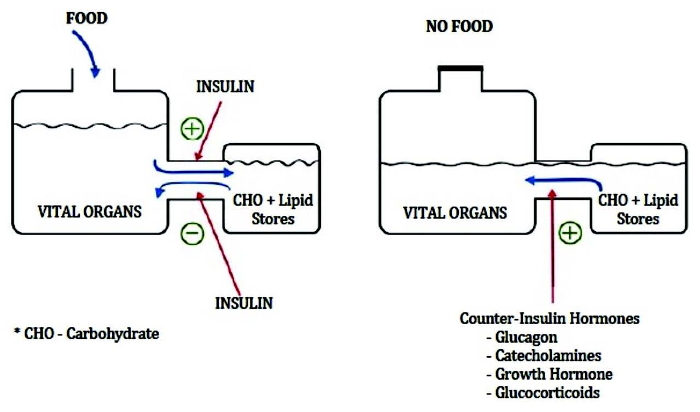
\includegraphics[scale=2.5]{images/017.jpg}\\
\textit{\textbf{Illustration of Glucose Homeostasis (equilibrium)}}
\end{figure}

After a meal, the vital organs utilize as much calories as they need. Excess calories are stored as fat (triglycerides) and carbobydrate\break (glycogen). During starvation, the stored calories are used to power\break vital organs. These changes are modulated by insulin \& counter–insu\-lin hormones.

The human body does a remarkable job of maintaining blood sugar levels between 80 mg per deciliter and 120 mg per deciliter at all times.
 This is despite several intrinsic (inside the body) and extrinsic (outside the body) factors that can both increase and decrease the blood sugar levels dramatically. For example, after a meal the blood sugar level is likely to shoot up due to the influx of glucose into blood. But the human body rapidly brings down the blood sugar levels to below 120 mg per deciliter. If blood sugar levels are more than 200 mg per deciliter 2 hours after a meal, it is diagnostic of diabetes. Thus, under normal conditions, the body takes less than 2 hours to normalize blood sugar levels after a meal induced surge.

\vskip 6pt
On the other hand, after a prolonged fast, or after rapid\break expenditure of calories (for example through vigorous exercise), the blood sugar level is susceptible to drop below 80 mg per deciliter. This condi\-tion is termed \textit{“hypoglycemia”\index{Hypoglycemia}}. The human brain can only use\break glucose as its energy source, and if the blood glucose levels drop\break below 80 mg per deciliter, there is a significant risk of the brain cells\break star\-ving and going into a condition known as \textit{“hypoglycemic coma”\index{Hypoglycemic Coma}}. It is both scary and hard to believe that every morning we wake up\break (after an overnight fast) at risk of hypoglycemic coma, but our body’s\break regulatory mechanism prevents this catastrophe.

\vskip 6pt
So how does the human body manage this incredible tightrope\break walk?

\vskip 6pt
It is by a phenomenon known as “glucose homeostasis”. This is a dynamic interplay of \textit{glucose, insulin, glucagon\index{Glucagon}}.

\vskip 6pt
As we know, all glucose in the body comes from the food we\break consume. However, different foods have different glucose content. Candy would obviously have more glucose than curry. All this\break glucose derived from food is absorbed into the blood stream.\break However, not a single milligram of glucose in the blood stream can\break enter the human cell without the help of insulin. Insulin acts as a key that unlocks the door to allow glucose enter the human cell. Once\break inside the cell, glucose powers the biochemical activities of the cell. Once the energy requirement of the cell is satisfied, what happens to the excess or leftover glucose inside the body? Insulin comes to the rescue again, and helps convert this surplus glucose into a storage form known as glycogen. Glycogen is stored mostly in the liver, and also in the muscles. \textcolor{blue}{Interestingly our liver has an ‘emergency fund’ of about 1/4 kilogram of sugar in the form of glycogen!}

\vskip 6pt
Now let us look at the flip side of the coin. If there is a shortage of glucose in the blood, as can happen with fasting, vigorous exercise etc, there is a risk of blood glucose levels plummeting below 80 mg/dl. When this happens there is a peril or great risk of the brain being\break deprived of fuel (glucose), and going into a coma. Each night when we go to bed and fast for 8 to 9 hours during sleep, we are in essence at risk of hypoglycemic coma! So how is this calamity prevented on a daily basis? We have to thank the hormonal action of glucagon for this.

\vskip 6pt
\textit{Glucagon\index{Glucagon}} is synthesized in the pancreas, and released into the blood stream whenever the blood glucose level dips below 80 mg/dl. It acts on glycogen, the stored form of glucose, present in the liver and muscle cells, and converts glycogen to glucose. Glucagon then acts as a key and unlocks the doors of the cell to allow glucose to exit into the blood stream.

\vskip 6pt
Thus, both insulin and glucagon act as keys. Insulin unlocks doors that allow glucose to enter the cell, while glucagon unlocks doors to allow glucose to exit the cell. This interesting and opposing action of insulin and glucagon is essential for blood glucose harmony. Any disruption in this delicate balance results in diabetes, which results in chronically elevated blood sugar levels. The excess sugar results in what are known as ‘advanced glycation end products or AGE’. These products accumulate inside cells and incite inflammation. This chronic inflammation eventually results in damage to the heart, kidneys, eyes, nervous system, skin, and reproductive organs.

\begin{figure}[h]
\centering
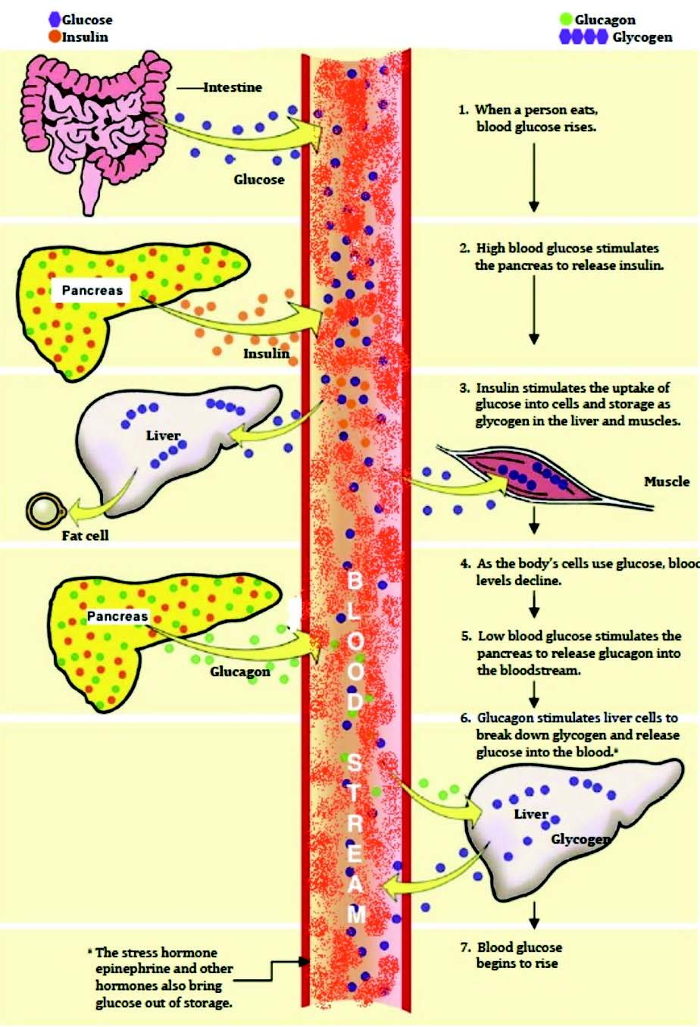
\includegraphics[scale=2.5]{images/018.jpg}\\
\textbf{\textit{Pictorial description of glucose metabolism}}
\end{figure}


\chapter{What is diabetes and how is it caused}\label{chap3}

Diabetes is an inherent inability to regulate the levels of glucose in\break the body. It is a disorder of carbohydrate, protein and fat metabolism.

\noindent
\textbf{Causes of diabetes}

Diabetes is a chronic condition. It is not exactly a disease, but\break a defect of insulin action, and a disorder of glucose metabolism. Unlike acute conditions such as a stroke or a heart attack that strike in a matter of seconds, diabetes typically takes 4 to 7 years for the insulin, glucose metabolism to completely derail, after which, excess glucose accumulates in blood and in different organs.

There are two main causes of diabetes:
\begin{enumerate}
\itemsep=0pt
\item Insulin deficiency
 \item Insulin resistance.
\end{enumerate}

Insulin deficiency occurs due to decreased production of insulin. This in turn is due to destruction of the insulin secreting beta\break cells in the pancreas. As per the available scientific knowledge, viral\break infe\-ctions and genetic factors are partly responsible for destruction of the beta cells. Insulin resistance is mediated by the hormone glucagon, which renders insulin ineffective. To overcome the resistance, the beta cells in the pancreas pump increasing amounts of insulin into the blood. But the body can only use a fraction of this excess insulin to meta\-bolize blood glucose. The blood glucose levels continue to stay at abnormally high levels in the body. On the other hand, the unused insu\-lin progressively accumulates in the tissues and becomes toxic. This is the stage of “insulin toxicity”, or the paradox of “insulin\break toxicity”. Insulin resi\-stance usually commences during adolescence, and continues throughout life. To keep up with the ever increasing\break demand for insulin, the pancreatic beta cells work overtime to\break produce increasing amounts of insulin. With the passage of time,\break the overworked pancreatic beta cells breakdown and start to die (by a process known as \textit{apoptosis} or cell death). This eventually depletes the total number of functioning beta cells. This negative chain of events conti\-nues to spiral out of control till all the beta cells in the pancreas become dysfunc\-tional, and there is an absolute lack of insulin in the human body. This process usually takes several decades. Hence this tends to manifest in the middle or older age groups. Lately however, we are increasingly witnessing this phenomenon in adolescents also!

In general, it is quite common to have both insulin deficiency\break and resistance simultaneously in diabetics. Either of these causes will ultimately result in insulin dysfunction. Insulin dysfunction will lead to disorderly metabolism of glucose, fat and protein.

The more one ponders over this concept, the more obvious it is that diabetes is a defect (of insulin) and a disorder (of metabolism), rather than a disease per se.

\noindent
\textbf{The dysfunction in diabetes at the level of the human cell}

Most of the glucose the body needs is derived from food, primarily from carbohydrates. Cells have to then convert glucose into energy. But glucose has to first gain entry inside the cell. Insulin is the hormone that makes this happen. Insulin is the key that unlocks the doors of the cell to allow glucose to enter inside. In technical terms, insulin binds to the receptors on the surface of the cell and “opens” the cell for glucose to enter inside. Without this key not a single molecule of glucose can enter the cell. This process is illustrated in the following pictures.

\begin{figure}[h]
\centering
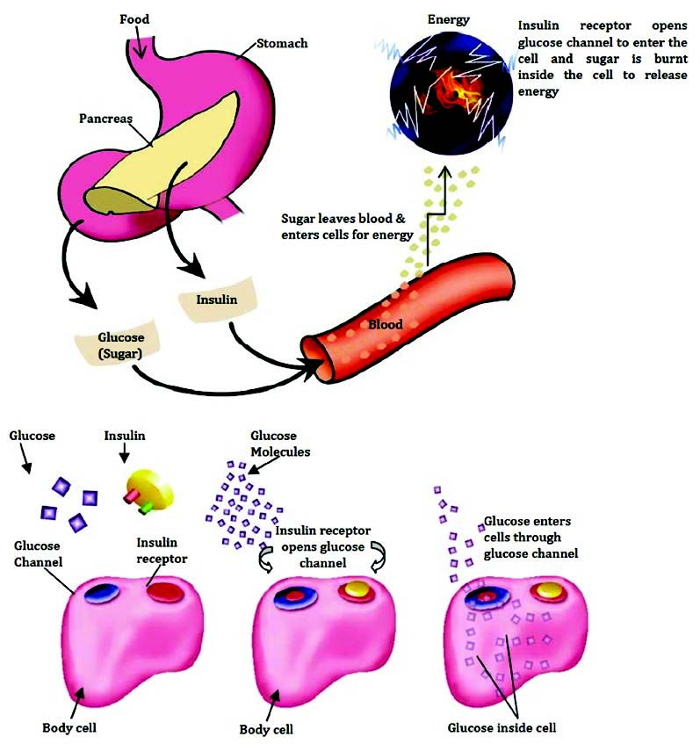
\includegraphics[scale=2.3]{images/019.jpg}\\
\textbf{\textit{Conversion of food to energy: The role of insulin}}
\end{figure}

\newpage
\noindent
\textbf{What goes wrong at the cellular level in diabetes?}

\begin{wrapfigure}{l}{4.5cm}
\vskip-.5cm
\centering

\includegraphics[scale=.6]{images/020.jpg}\\
\textbf{\textit{Insulin–key to\\ open the cell}}
\vskip-.6cm
\end{wrapfigure}

In people with type 1 diabetes, the key (insu\-lin) is missing (no insu\-lin produ\-ction). This happens when the islets (specifically the insulin\break producing beta cells) of the pancreas are destroyed.

\clearpage
In people with type 2 diabetes, the key (insu\-lin) does not fit. This phenomenon where there’s plenty of insu\-lin but the body cannot use it pro\-perly, is known as insulin resistance. This same pheno\-menon also\break occurs in gestational diabetes mellitus (GDM), a type of diabetes that occurs in pregnancy. Gestational diabetes usually resolves after childbirth, although women who develop GDM have a higher risk for\break developing the permanent insulin resistance of type 2 diabetes later in life.

\vskip 20pt

\begin{figure}[h]
\centering
\textbf{\textit{An illustration of insulin resistance}}
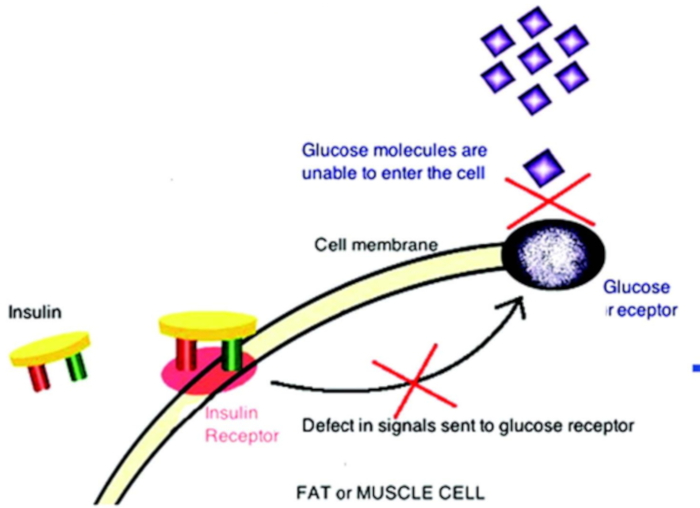
\includegraphics[scale=2.5]{images/021.jpg}
\end{figure}

\clearpage

\textbf{}
\begin{figure}[h]
\centering
\textbf{In short how is diabetes caused?}\\
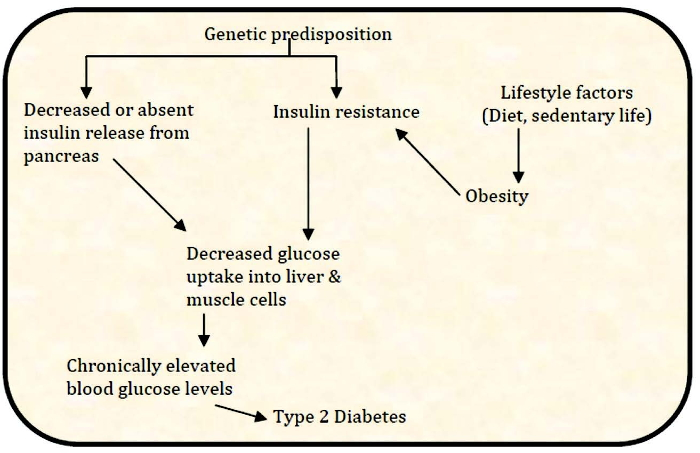
\includegraphics[scale=2.6]{images/022.jpg}
\end{figure}


\chapter{Signs and symptoms of diabetes}\label{chap4}

The following are the usual manifestations of diabetes:

\begin{figure}[h]
\centering
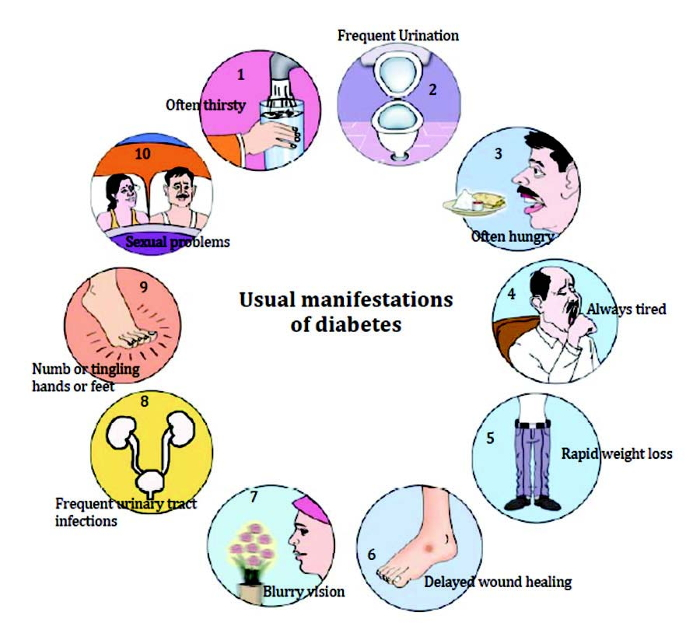
\includegraphics[scale=2.3]{images/023.jpg}
\end{figure}

In addition, diabetics may also have the following symptoms:

\begin{enumerate}[\ding{226}]
\itemsep=0pt
\item Increased sweating while eating
\item Repeated skin infections
\item Decreased sensation in feet
\item Frequent episodes of urinary tract infections
\item Feeling dizzy
 \end{enumerate}

However, not every diabetic will have all these symptoms. The\break exact constellation of symptoms may differ from person to person. Even a single symptom is enough to suspect diabetes. However, up to 50\% of diabetics may not have any obvious symptoms or signs of diabetes. So how do these people get diagnosed with diabetes? They\break usually come to light when blood tests show high blood sugar levels during routine health check ups for either health insurance scree\-ning, or life insurance screening, or when they present to the hospital for an un\-related reason such as a minor wound, cataract surgery etc. But if they never present to a hospital for any reason, they may remain undia\-gnosed. Even these so called asymptomatic diabetics will have mild symptoms such as unintentional weight loss, minor skin infections, itching in the private parts etc. Unfortunately, these undiagno\-sed dia\-betics are likely to eventually come to medical attention with a compli\-cation such as a heart attack, stroke, vision loss, coma etc. This is because, while they remain undiagnosed, the high blood sugar silently but relentlessly, damages the body, similar to termites eating away a tree from the inside. For this reason, it is important to screen indi\-viduals for diabetes at routine intervals.

\noindent
\textbf{What are the reasons behind the different symptoms of diabetes?}

Have you ever wondered why people with diabetes have the symptoms described above?

\noindent
\textbf{What causes increased hunger or \textit{polyphagia?\index{Polyphasia}}}

Glucose is the fuel that powers all activity inside the human cell. However, just as all the water of the sea cannot quench human thirst, the excess sugar in the blood of a diabetic cannot meet the energy needs of the human cell. This is because insulin is fundamental for the glucose molecules to gain entry inside the human cell.

Thus, even though the human cell is bathed in sweet blood, it is starved of energy. Hence the body craves for energy and this causes increased hunger.

\noindent
\textbf{What causes increased weight loss?}

Unable to utilize glucose, the body resorts to breaking down the body’s fat reserves to use as energy for its cells. This results in weight loss. Lack of adequate fuel for cells to function can also result in dizziness.

\noindent
\textbf{What causes increased urination or \textit{polyuria?\index{Polyurea}} What causes excess thirst or \textit{polydypsia?\index{Poly dypsia}}}

The excess blood sugar overwhelms the kidney’s filtration capa\-city. Once the blood sugar level exceeds 180 mg/deciliter, sugar starts to spill out into urine. In order to keep this excess sugar in the urine in a dissolved state, the body has to pump excess water into urine. This results in excess urination, and excess thirst (from excess fluid loss through urine).

\noindent
\textbf{What causes repeated infections?}

High blood sugar levels offer a favorable environment for microbes (bacteria, viruses, fungi) to thrive, and this causes repeated infections.

\noindent
\textbf{Identifying signs of diabetes in children and adolescents: Role of parents and caretakers}

Children and adolescents with diabetes present unique challenges. Unlike adults who are able to identify their symptoms, express them and seek medical care, children and adolescents may be unable to pro\-perly identify the changes their bodies undergo due to diabetes. Thus, the onus of early diagnosis and management falls on their parents. In addition to the usual symptoms and signs described earlier in this chapter, diabetic children exhibit some unique features such as:

\begin{enumerate}[\ding{226}]
\itemsep=0pt
\item Impaired growth despite getting seemingly adequate nutrition
\item Ants making a beeline for the child’s urine!
\item Frequent infections
\item Unexplained loss of consciousness
\end{enumerate}

It is important for parents not to lose heart when their dear ones are newly diagnosed with diabetes. It has been shown that prompt treatment with insulin will result in a normal lifespan, an energetic life, ability to procreate and bear children, and fewer complications of diabetes.

\textcolor{blue}{\textit{it is important to avoid dietary restrictions in diabetic children!}} Unlike adults, where diet is an integral part of managing diabetes, children should be allowed to eat as they please, since they need high nutrition to maintain normal growth. To counter the increased blood sugar that may result from eating an unrestricted diet, necessary doses of insulin should be administered.



\chapter{Diagnosing diabetes}\label{chap5}

There are 3 objectives of diagnosing diabetes:

\begin{enumerate}
\itemsep=0pt
\item To confirm the presence of diabetes, so that it can be treated
\item To differentiate the type of diabetes (type 1 versus type 2)
\item To aid in calculating the incidence and prevalence of diabetes in the country. This important statistics helps estimate the disease burden in the country/world. Based on this information, appropriate allocation of funds and manpower is made to curb the disease and its impact on society.
\end{enumerate}

For readers’ information, incidence refers to new cases of a parti\-cular disease in a particular population. Prevalence refers to all or the total number of cases of a particular disease – both new and old, in a particular population.

\noindent
\textbf{Diagnostic test for diabetes}

Any test that is used to diagnose a disease that is both common and chronic should have the following characteristics:

\begin{enumerate}[a.]
\itemsep=0pt
\item The test should be simple i.e. it should be quick, and people should not require extensive technical training to perform this test.
 \item The test should be cheap, so that it can be performed in every corner of the globe.
 \item The test should be accurate and reliable.
 \item The test should be standardized, meaning that the way the test is performed and interpreted should be the same in any part of the world.
 \item The test should be able to prognosticate or predict the outcome of a chronic disease such as diabetes.
 \end{enumerate}

Keeping these criteria in mind, in 1979 the World Health Organi\-zation (WHO), in association with the National Diabetes Data Group, developed the oral glucose tolerance test (OGTT) to diagnose diabetes$^{\text{\cite{chap5–key01}}}$.

\noindent
\textbf{Oral Glucose Tolerance Test (OGTT)}

The oral glucose tolerance test involves giving an individual 75 gm of glucose to consume, and measuring the blood sugar level 2 hours later. According to this test, either a fasting blood glucose level of 140 mg per deciliter, or a blood glucose level more than 200 mg per deciliter 2 hours after consuming 75 gm of sugar was considered to be diagnostic of diabetes.

These guidelines were updated in 1997 by the American Diabetic Association (ADA), and later revised in 2003. As per the new guidelines, any one of the following three criteria is required to diagnose diabetes$^{\text{\cite{chap5–key02}}}$.:

\begin{enumerate}
\itemsep=0pt
\item A fasting blood sugar level of 126 mg per deciliter or higher + symptoms of diabetes. (Fasting blood glucose is measured after an 8–hour fast)
\item A random (meaning anytime, fasting or otherwise) blood sugar level of 200 mg per deciliter or higher.
\item A blood sugar value of 200 mg per deciliter or higher 2 hours after OGTT (oral glucose tolerance test).
 \end{enumerate}

\noindent
\textbf{Predicting the future}

Blood sugar levels are not only diagnostic of diabetes, but research has shown that they can predict the future course of the disease. Three blood sugar values are of particular significance when it comes to\break predicting the future of patients with diabetes or individuals at risk for diabetes:

\begin{enumerate}
\itemsep=0pt
\item A random blood sugar level above 200 mg per deciliter is shown to be associated with higher risk of long–term complications of diabetes involving the eyes, heart, nervous system, kidneys and blood vessels.
 \item A fasting blood glucose level between 100 to 125 mg per deciliter is termed impaired fasting glucose (IFG)
 \item A blood sugar level between 140 to 200 mg per deciliter 2 hours after the OGTT is termed impaired glucose tolerance (IGT).
 \end{enumerate}

Individuals who have either impaired fasting glucose (IFG) or\break impaired glucose tolerance test (IGT) are referred to as having “prediabetes”. Prediabetes is a condition where the glucose metabolism is faulty, but not abnormal enough to qualify as full–blown diabetes.

\noindent
\textbf{What does it mean to have \textit{prediabetes?\index{Prediabetes}}}

The prediabetes state is a strong predictor of the eventual deve\-lopment of diabetes.

Based on studies among individuals with prediabetes:

\begin{enumerate}[a)]
\itemsep=0pt
\item A fasting blood glucose level of 100 to 110 mg per deciliter is asso\-ciated with an 8.1\% risk of developing diabetes in the next 10 years.
 \item A fasting blood glucose level of 110 to 125 mg per deciliter is associated with a 24.3\% risk of developing diabetes in the next 10 years.
 \end{enumerate}

\textcolor{blue}{\textit{Thus, for the first time in the history of diabetes, we are able to identify patients before they develop diabetes.}} Targeting this high–risk group has the potential to prevent the eventual onset of diabetes. This has major implications in the battle against diabetes! This is described in greater detail later in the book.

\noindent
\textbf{A newer method of diagnosing diabetes}

The fasting glucose levels, and 2–hour post–meal blood glu\-cose le\-vels proposed by the World Health Organization are universally ado\-pted in diagnosing diabetes. Of late, there has been much deliberation at the international level about simplifying the diagnosis of diabetes. The American Diabetic Association (ADA) is recommending that\break fasting blood glucose alone is enough to make the diagnosis of diabetes.


An international expert committee comprising members appoin\-ted by the ADA, EASD (European Association for Study of Diabetes), and IDF (International Diabetes Foundation) was established to look into newer means of diagnosing diabetes. In 2008, the expert commi\-ttee came out with its recommendation that a HbA1c level greater than 6.5\% was diagnostic of diabetes and could be used as another test to\break diagnose diabetes$^{\text{\cite{chap5–key04}}}$.

HbA1c or Hemoglobin A1c is described in greater detail later in this book.

\begin{thebibliography}{99}
\bibitem{chap5–key01} Classification and diagnosing diabetes and other categories of\break glucose intolerance. National Diabetes Data Group. Diabetes 1979; 28 (12): 1039–1057
 \bibitem{chap5–key02} Genuth S, Alberti KG, Bennett P, Buse J, et al. Follow–up report on the diagnosis of diabetes mellitus. Diabetes Care 2003; 26 (11): 3160–3167
 \bibitem{chap5–key03} Nichols GA, Hillier TA, \& Brown JB. Progression from newly\break acquired impaired fasting glucose to type 2 diabetes. Diabetes Care. 2007; 30: 234–238.
 \bibitem{chap5–key04} Gillett MJ. International expert committee report on the role of A1c assay in the diagnosis of diabetes. Diabetes Care 2009; 32:1327–34
 \end{thebibliography}


\chapter{Types of diabetes}\label{chap6}

There are two main types of diabetes.

Type 1 diabetes predominantly occurs in children.

Type 2 diabetes predominantly occurs in the middle–aged popu\-lation.

In addition, “gestational diabetes mellitus” (GDM) is seen in pregnant women.

As per the latest research two more types of diabetes are added. They are:

\begin{enumerate}[-]
\itemsep=0pt
\item Monogenic Diabetes Syndromes – MODY type
\item Chemical induced diabetes
\end{enumerate}

\begin{wrapfigure}{r}{4cm}
\centering
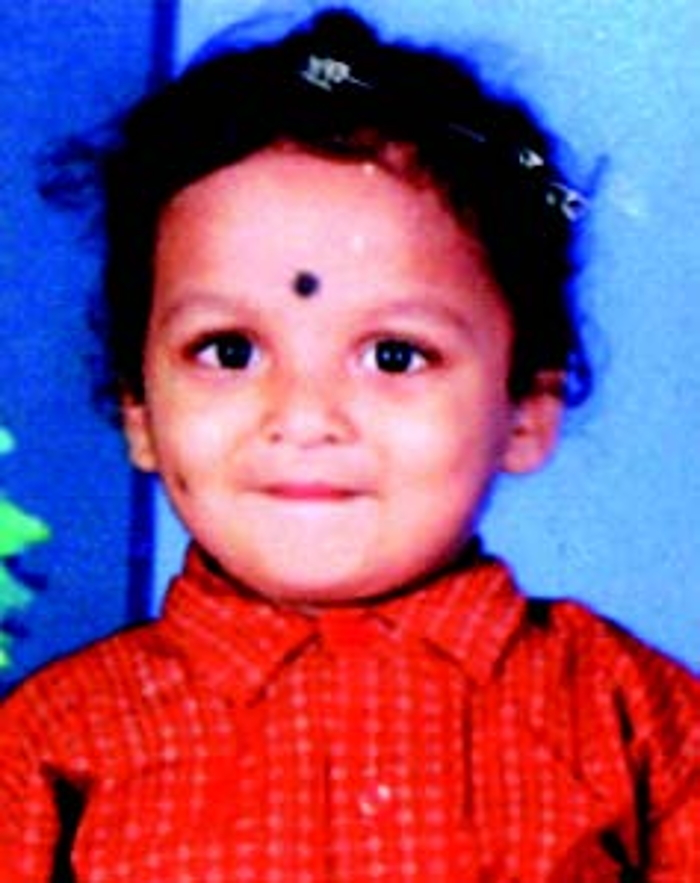
\includegraphics[scale=.5]{images/024.jpg}\\
{\small\textbf{\textit{Type 1 diabetic child\\ on daily insulin}}}
\vskip-.5cm
\end{wrapfigure}

MODY is maturity onset diabetes of the young, which is due to genetic defects of B–cell function. 13 such defects are identified in MODY.


Type 2 diabetes is the predominant type and accounts for 90–95\% of all diabe\-tics worldwide. Type 1 diabetes accounts for 5–10\% of diabetics worldwide.

\noindent
\textbf{Type 1 Diabetes}

This type of diabetes is also known as \textit{“juvenile diabetes”\index{Juvenile diabetes}}, since it mainly affects children and adolescents. In this type of diabetes, there is an absolute lack of insu\-lin. Daily insulin injections are essential for survival of these individuals.

\noindent
\textbf{Type 2 Diabetes}

While this disease can affect anybody, three groups are especially predisposed– the obese, those who consume high calorie foods, and the middle–aged. Genetic predisposition and obesity lie at the root of this disease.

Genetic predisposition puts the individual at increased risk to\break develop diabetes even as the fetus is still in the uterus! If the mother is diabetic, the growing fetus has an increased risk of developing defe\-ctive beta cells in the pancreas. Also the child is more likely to be obese and to develop insulin resistance$^{\text{\cite{chap6–key01}}}$. Diabetes lies dormant in these genetically predisposed individuals. A lethargic lifestyle eve\-ntually sparks full–blown diabetes. It is possible to identify this genetically predisposed high–risk group by means of a test called the \textit{“Glucose\break Challenge Test” or “GCT”}\index{Glucose challenge test (GST)}. In this test, glucose is injected into the veins and serial blood sugar levels are measured. In a genetically predisposed individual, the body struggles to handle a sudden load of sugar. This can be objectively demonstrated by measuring the blood sugar and insulin levels. Such individuals are likely to develop diabetes.

\textit{Obesity\index{Obesity}} begins to lay the foundation for future diabetes, at a very early age. Studies show that low birth weight babies overfed by their anxious parents results in childhood obesity. Childhood obesity is asso\-ciated with a high risk of developing diabetes in adulthood.

\noindent
\textbf{\textit{Study showing the impact of Genetic Predisposition}}

An experiment was conducted to compare the prevalence of diabetes and the age–of–onset of diabetes between Indians (residing both in India and in USA), and people of European descent.

As part of the experiment, subjects were given 75 gm of glucose to consume, and their blood sugar levels were measured at timed intervals (this is nothing but the oral glucose tolerance test or OGTT, used to diagnose diabetes).

It was found that 50\% of people of European descent developed\break diabetes after crossing the age of 70 years.

However, among Indians this high rate of diabetes (50\%) was seen in people aged between 50 to 60 years, or in other words 10 years sooner than Europeans!

This intriguing study demonstrates some very worrisome facts:

\begin{enumerate}[a)]
\itemsep=0pt
\item People of Asian Indian race tend to develop diabetes 10 years earlier in life than their European counterparts.
\item Indians are at risk of developing diabetes early whether they reside in India or migrate to Western countries.
\end{enumerate}

\setlength{\parskip}{.2em}
\noindent
\textbf{\textit{Gestational Diabetes Mellitus (GDM)}}\index{Gestational diabetes mellitus}

Some pregnant women will have increased blood sugar levels. This condition is known as “Gestational Diabetes Mellitus”. It is estimated to affect 18\% of all pregnancies according to the American Diabetes Association. Generally gestational diabetes manifests in the 2nd to 4th month of pregnancy. This is a consequence of hormonal changes\break associated with pregnancy. These pregnant women may need insulin injections during pregnancy, to ensure a safe and uncomplicated\break pregnancy and delivery. This condition usually normalizes after deli\-very. However, these individuals are at higher risk for developing Type 2 diabetes by middle age. Hence, these women should check their blood sugar levels every 6 months to enable prompt diagnosis.

Recently it is recommended that they need to get blood glucose levels tested 4 to 12 weeks after delivery.

\setlength{\parskip}{.2em}
\begin{thebibliography}{99}
\bibitem{chap6–key01} Plagemannn A, Harder T, Franke K, \& Kohlhoff R. Long–term\break impact of neonatal breast feeding on body weight and glucose\break tolerance in children of diabetic mothers. Diabetes Care. 2002; 25(1): 16–22.
\end{thebibliography}


\chapter{Type 2 diabetes in children}\label{chap7}

In general type 1 diabetes affects children and adolescents. Type 2 diabetes on the other hand, usually affects adults. But you would be heartbroken to know that a child as young as 9 years of age was diagnosed with type 2 diabetes in Chennai, almost 40–50 years ahead of the usual time of onset of this disease. I have personally witnessed this tragic phenomenon when a 15–year old in our clinic was diagnosed with type 2 diabetes.


Imagine the implications of this phenomenon. The typical patient with type 2 diabetes is 40 to 60 years old at the time of diagnosis. By 50 to 70 years of age, the patient is likely to fall victim to crippling compli\-cations such as heart disease, stroke, kidney failure requiring dialysis, loss of vision, sexual dysfunction etc. But if a child is dia\-gnosed with type 2 diabetes by age 9, then by age 20 to 30 he or she would have suffered a heart attack, stroke, kidney failure, or lost vision or sexual function! Is this not heartbreaking for any parent to witness? And what about the serious implications for the country? The young soldier gua\-rding our borders who cannot use his hands due to stroke, or cannot see the enemy due to vision loss, or the young computer professional who has to miss work to have dialysis for kidney failure. India’s eco\-nomy could come to a grinding halt !


But are we overreacting to few case reports of type 2 diabetes\break among children, or are we just seeing the tip of the iceberg of a\break systemic rot?

\setlength{\parskip}{.5em}
A 10–fold increase in the number of children diagnosed with type 2 diabetes was reported by New York Medical Center, between 1990 and 2000.$^{\text{\cite{chap7–key01}}}$ In fact, the American Diabetes Association predicts that\break type 2 diabetes might become the most common form of newly\break diagnosed diabetes in adolescents.

\noindent In India the magnitude of this distressing trend is increasing.

\begin{enumerate}[•]
\itemsep=0pt
\item Researchers at Cochin, Kerala, reported type 2 diabetes in 6\% of young diabetics below the age of 20, compared to 89\% with type 1 diabetes.$^{\text{\cite{chap7–key02}}}$
\item Sanjay Gandhi Institute, Lucknow found type 2 diabetes in 8\% of dia\-betics below the age of 18 years.$^{\text{\cite{chap7–key03}}}$
\item The Madras Diabetes Research Foundation in Chennai reported type 2 diabetes in 26.7\% of diabetics under the age of 6 years.$^{\text{\cite{chap7–key04}}}$
\item In a 2007 study from the United Kingdom, Indian kids were found to have a 11 times higher rate of type 2 diabetes than White kids, and a 3 times higher rate than Black children.$^{\text{\cite{chap7–key05}}}$ This is due to the Asian Indian phenotype.
 \end{enumerate}


\textcolor{red}{\textit{The conclusions we can draw from these recent studies are that, type 2 diabetes is increasing at an alarming rate worldwide among kids, and Indian kids in particular have a significantly higher risk!}}

\noindent\textbf{Reasons for this alarming trend}


While we have talked about the causes for diabetes in adults in great detail in earlier sections of the book, there are certain novel factors that play a crucial role in children who develop type 2 diabetes. They are detailed below:

\noindent\textbf{A) Obesity:}

Children and adolescents were universally obese or overweight in majority of the studies of type 2 diabetes from the U.S. and U.K. I am sure every reader has seen the explosion of obesity in our kids in India as well. There are several reasons for this:

\begin{enumerate}[•]
\itemsep=0pt
\item Fast food culture : high sugar, high fat, high salt diets being eagerly gulped by our kids in the name of “Happy Meals” at McDonalds and their like.
\item Addiction to the television : In an interesting study from Harvard University, people who watched TV for more than 20 hours a week were twice as likely to develop diabetes compared to those who\break watched only 1 hour per week.$^{\text{\cite{chap7–key06}}}$ How often did you have to turn on the TV to make sure your kid eats his/her dinner? You may be surprised and even shocked to find out how many hours of TV your kids watch every week!
\item Sedentary life : TV watching and video games have replaced physical games we used to play in parks and playgrounds that are now making way for high rise buildings all over the country.
 \end{enumerate}

\noindent\textbf{B) Metabolic syndrome:}

Kids need not necessarily be obese to develop type 2 diabetes. In a 2003 study from Chennai, only 50\% of children with type 2 diabetes were obese. But more than 90\% had abdominal obesity.$^{\text{\cite{chap7–key07}}}$

Abdominal obesity (increased waist–to–hip ratio) is part of the\break metabolic syndrome that is unique to the “Asian Indian phenotype” described in the previous chapter. Other features of this phenotype include abnormal cholesterol pattern, high blood pressure, and insulin resistance.


\noindent\textbf{C) Family history:}

Heredity is a strong predisposing factor. In fact, up to 74–100\% of children and adolescents with type 2 diabetes have another family member with diabetes.



\noindent\textbf{D) Early life events:}

\begin{figure}[h]
\centering
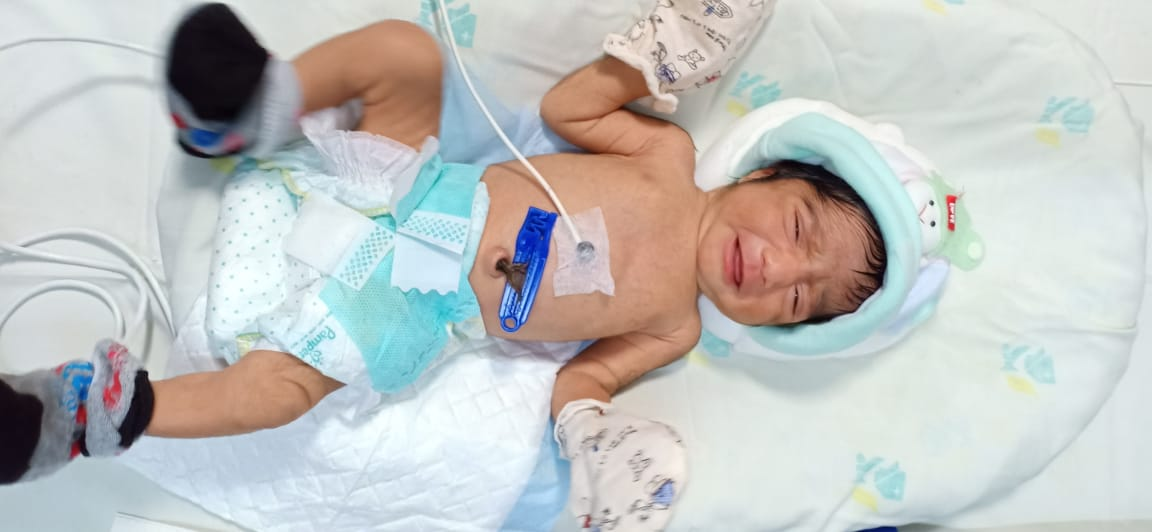
\includegraphics[scale=1.2]{images/025.jpg}\\
\small\textbf{\textit{Low birth–weight baby}}
\end{figure}

Indian babies frequently have low birth weight due to poor maternal nutrition during pregnancy, and inadequate breast–feeding during infancy. This is followed by a phase of catch–up growth in early life due to overfeeding of the kid by overzealous parents. These factors lead to insulin resi\-stance, and eventually to type 2 diabetes.

\noindent\textbf{Management of Type 2 Diabetes in children and adolescents}

Management of this condition presents several extraordinary\break challenges:

\noindent\textbf{A) Non–specific or vague symptoms:}

Unlike type 1 diabetes, children with type 2 diabetes seldom have the classic ‘polys’ of diabetes namely– polydypsia, polyuria, etc. They are also less likely to lose weight rapidly.

They are more likely to manifest subtle (delicate) symptoms such as increasing fatigue, lack of interest in life, dropping grades/marks in school etc. For parents and teachers dealing with a teenager’s emotional ups and downs, picking up subtle signs of early diabetes can be extremely difficult. This can lead to delays in diagnosis of the disease.

\noindent\textbf{B) Accelerated complications of diabetes:}

Studies show that kidney damage, vision loss, and cardiovascular complications happen faster in type 2 diabetic adolescents compared to type 1 diabetics. In combination with the delay in diagnosis as explained above, this aggressive nature of disease can clip the wings of our youth even before they take flight.

\noindent\textbf{C) Non–compliance with treatment:}

It takes a great deal of patience on part of both the parents and pediatricians who care for young diabetics. The children are usually oblivious to the seriousness of the disease, and adolescents are often rebellious. Many end up profoundly deeply depressed as well due to the stress of having diabetes.


\noindent\textbf{Management strategies}

The cornerstone of management is prevention. This requires a multi–pronged approach involving parents, teachers, pediatricians,\break media, non–governmental organizations (NGOs), and the government.

\noindent\textbf{\textit{Screening high risk groups}}

The most cost–effective preventive intervention would be to\break identify high–risk groups and screen them for diabetes and pre–dia\-betes, and initiate further care. High–risk groups include those children and adolescents with

\begin{enumerate}[•]
\itemsep=0pt
\item Family history of diabetes
\item Obesity
\item Tendency to eat junk food
\item Acanthosis nigricans – a skin disorder in which there is dark, velvety skin in the armpits, groin, neck folds, over the joints of fingers and toes. This identifies individuals with insulin resistance and a predisposition to type 2 diabetes. About 10–20\% of obese children are found to have Acanthosis nigricans

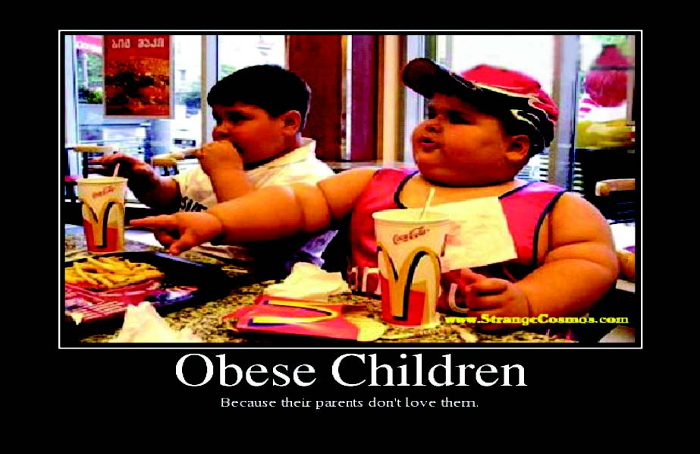
\includegraphics[scale=1.2]{images/026.jpg}\\
\small\textbf{\textit{Junk food and obesity in children}}

\item Metabolic syndrome – identified by measuring the waist–to–hip\break ratio, cholesterol levels in blood, and blood pressure.
\item Polycystic ovary syndrome (PCOS) – this is a state of hormonal\break imbalance among women. This results in irregularities of the menstrual cycles (decrease or absence), male characteristics (hair growth, deep voice) and worsening acne. This condition results in insulin resi\-stance, and hence predisposes to type 2 diabetes.
\end{enumerate}

\noindent\textbf{\textit{Populationwide interventions}}

In addition to focused screening as explained above, we need to educate the society in general about this growing problem. In a study conducted in Chennai, only 25\% had heard of diabetes, and more than 75\% did not know that the disease could be prevented (Deepa M et al. J Assoc Physicians India 2005; 53: 283–87).

\noindent
At the parental level–

\begin{enumerate}[•]
\itemsep=0pt
\item Closely monitor your child. Does he/she seem unusually lethargic; are the grades in school dropping etc?
\item Ensure adequate physical activity
\item Cut down the hours spent in front of TV or playing video games
\item Avoid going to fast food joints
\item Set an example for your child by doing all the above yourself!
\end{enumerate}

\noindent
At the school level–

\begin{enumerate}[•]
\itemsep=0pt
\item Pay attention to your pupils’ outward behavior and their grades\break in class
\item Ensure enough outdoor space for the kids to play
\item Ensure at least 1 hour of physical training during the day
\item Encourage annual school–wide medical check–ups including\break blood and urine tests. This may require coordination with medical NGOs.
\end{enumerate}

\noindent
At the society level–

\begin{enumerate}[•]
\itemsep=0pt
\item Plan to have parks and playgrounds that are accessible for the kids in the neighborhood
 \end{enumerate}

\clearpage

\noindent At the government level–

\begin{enumerate}[•]
\itemsep=0pt
\item Initiate measures to prevent malnutrition during pregnancy and\break lactation
 \item Use mass–media (TV, radio, print media) to spread awareness about the disease.
 \end{enumerate}

\begin{thebibliography}{99}
\bibitem{chap7–key01} Grinstein G, Muzumdar R, Aponte L, Vuguin P, Saenger P, \&\break Dimartino. Nardi J. Presentation and 5–year follow–up of type 2 diabetes in African American and Carribean–Hispanic adole\-scents. Horm Res. 2003; 60 (3): 121–6.
 \bibitem{chap7–key02} Unnikrishnan AG, Bhatia E, Bhatia V, Bhadada SK, et al. Type 1 dia\-betes versus type 2 diabetes with onset in persons younger than 20 years of age. Ann N Y Acad Sci. 2008; 1150:239–44
 \bibitem{chap7–key03} Bhatia V, Arya V, Dabadghao P, Balasubramanian K, et al. Etio\-logy and outcome of childhood and adolescent diabetes mellitus in North India. J Pediatr Endocrinol Metab. 2004; 17(7): 993–9.
 \bibitem{chap7–key04} Mohan V, Jaydip R, \& Deepa R. Type 2 diabetes in Asian Indian youth. Pediatr Diabetes. 2007; 8 Suppl. 9: 28–34.
 \bibitem{chap7–key05} Haines L, Wan KC, Lynn R, Barrett TG, \& Shield JP. Rising incidence of type 2 diabetes in children in the U.K. Diabetes Care. 2007; 30 (5):1097–101.
 \bibitem{chap7–key06} Hu FB, Leitzmann MF, Stampfer MJ, Colditz GA, et al. Physical\break activity and television watching in relation to risk for type 2 diabetes mellitus in men. Arch Intern Med. 2001; 161 (12): 1542–8.
 \bibitem{chap7–key07} Ramachandran A, Snehalatha C, Satyavani K, Sivasankari S, \&\break Vijay V. Type 2 diabetes in Asian–Indian urban children. Diabetes Care. 2003; 26 (4): 1022–5.
 \end{thebibliography}


\chapter{Diabetes in India}\label{chap8}

\noindent\textbf{India – the erstwhile diabetes capital of the world}

India has consistently earned the dubious distinction of having the largest number of diabetics in the world. It had held this top spot since 1980 as per the World Health Organization (WHO) data! Only recently has it conceded this top spot to China.

For us to be able to reverse this epidemic, we need to first examine the history, demography and the causes of the epidemic.

\noindent\textbf{History of diabetes in India}

Before gaining independence in 1947, diabetes was a rare disease. It was mostly a disease of the rich and famous, thought to be a con\-sequence of their lavish and sedentary lifestyle.

But over the past few decades, the disease has spread its tentacles to every level of our society, affecting the rich and poor, urban and rural–dwellers, young and old, man, woman, and child. Consequently the number of Indians suffering from diabetes has exploded. Please see Chapter \ref{chap9} – Diabetes – Global Picture.

A closer look at the trend shows that majority of the increase in numbers has happened in the past few decades as seen in serial prevalence studies conducted in Chennai. Please see Chapter \ref{chap9} – Diabetes – Global Picture.

According to these figures, between 1989 and 2004, there has been a 72.3\% increase in prevalence in diabetes!

Based on these kinds of studies the International Diabetes Federation and the World Health Organization predict similar rates of growth in diabetes prevalence in India over the coming years. Please see\break Chapter \ref{chap9} – Diabetes – Global Picture.

\noindent\textbf{Demography of diabetes in India}

Demography is the study of a whole population (instead of a single person). Demography can give us very useful information regarding disease trends. For example, it can tell us if diabetes is more common in urban versus rural areas, South India versus North India, middle–age group versus older age, male versus female etc. Let us now examine some of these demographic features of diabetes in India.

\noindent\textbf{Diabetes prevalence in urban versus rural India}

Diabetes certainly started off being a disease of the urban elite. It continues to be more common in urban areas. However, there are increasing numbers of diabetics in rural areas too. According to a study jointly conducted in 2006 by the WHO and ICMR in five different states located in five different geographical locations (North, South, East, West and Central India) the prevalence of diabetes in urban areas is 7.3\%, and rural areas it is 3.1\%.

\noindent\textbf{Geographic distribution of diabetes in India}

India has always been a country of diverse cultures, languages etc. The prevalence of diabetes in India is also very diverse. The highest prevalence is among South Indians, with some places such as Ernakulum in Kerala having 2–3 times the rate in New Delhi or the Kashmir valley. Several reasons can explain this difference:

\begin{enumerate}[•]
\item Predominant rice–based diet in the South: Rice tends to raise the blood sugar more than wheat, which is the staple diet in the North.
\item Genetic differences.
\item More frequent screening for diabetes due to higher urbanization in the South.
\end{enumerate}

\begin{figure}[h]
\centering
\textbf{Map of India with prevalence rates of diabetes}\\
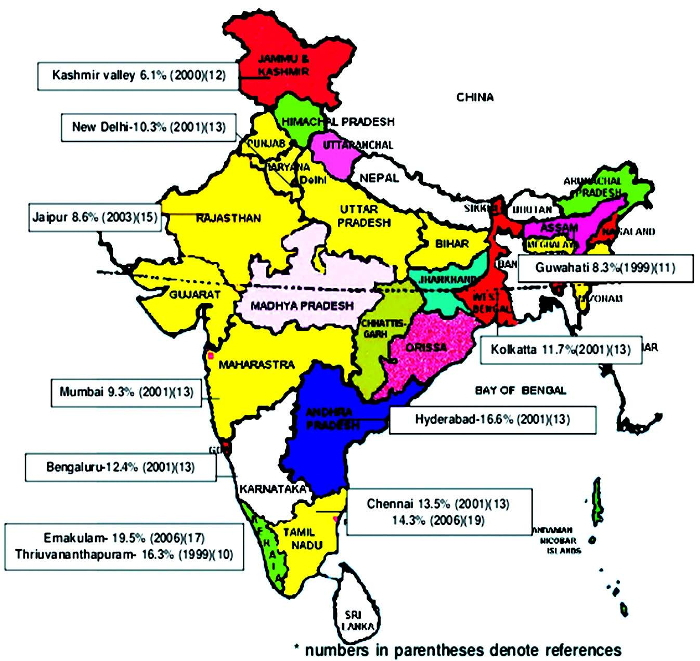
\includegraphics[scale=2.4]{images/027.jpg}\\
\textbf{Note: Kerala tops list of Indian States followed by Tamil Nadu and Punjab}
\vskip-.5cm
\end{figure}

Oddly the opposite trend is seen in developed countries. For\break example in Australia, the prevalence in urban areas was 7.4\% versus 11.6\% in rural areas.$^{\text{\cite{chap8–key01}}}$


\noindent\textbf{Age distribution of diabetes}

An alarming trend is emerging in India. Type 2 diabetes is\break being diagnosed at a much younger age; in fact, many decades\break earlier than expected. While physicians across the country are\break witnessing this phenomenon in their clinics, this was systematically demonstrated by comparing two major studies. The National Urban Dia\-betes Survey (NUDS) was conducted in 2000, and the Chennai Urban Rural Epidemiology Study (CURES) was conducted in 2004.

\begin{figure}[h]
\centering
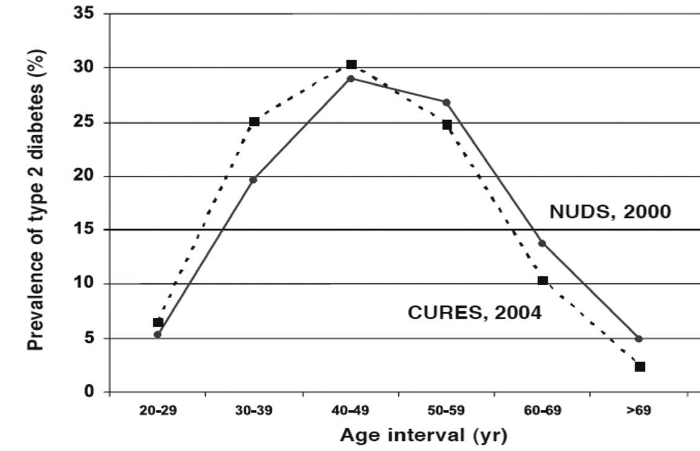
\includegraphics[scale=2.4]{images/028.jpg}\\
\small\textbf{\textit{Newly diagnosed type 2 diabetics were younger in 2004 compared to 2000}}
\vskip-.5cm
\end{figure}

\noindent\textbf{Causes of the diabetes epidemic in India}

The causes of this disturbing phenomenon in our country can be analyzed under 3 broad categories, namely genes, lifestyle, and\break epidemiologic transition.

\noindent\textbf{Genes}

Some diseases tend to run in families. So if parents have diabetes or heart disease, then their offspring is at the risk of developing these conditions. This is a well–known fact in our culture. In fact, in the elaborate matchmaking process of an arranged marriage, the elders of both fami\-lies meet each other at the bride’s home to secretly examine for any evidence of diseases of the body or mind in the other family!

The risk of acquiring diabetes in the offspring based on family\break history of diabetes is shown in the table below:

\begin{center}
\begin{tabular}{|l|l|}
\hline
& Offspring’s risk of\\
& developing diabetes\\
\hline
Both parents are diabetic & 90\%\\
\hline
One parent is diabetic & 70\%\\
\hline
Any family member is diabetic & 40\%\\
\hline
\end{tabular}
\end{center}

While we are yet to identify the exact genes that increase the risk of diabetes in Indians, several research studies consistently demonstrate the elevated risk of diabetes among Indians. This high–risk genetic make–up operates in certain unique ways listed below:

 \begin{enumerate}
 \itemsep=0pt
\item \textbf{Higher glycemic response:} Glycemic response is the amount of increase in blood glucose after food intake. In a study comparing the British and Indians, it was found that for the same calorie intake, Indians had a higher blood sugar level than the British.$^{\text{\cite{chap8–key02}}}$
\item \textbf{Increased abdominal obesity:} This is defined as the increased ratio of waist circumference to the hip circumference (picture a pot–belly). We are in general not more obese than the Cauca\-sian or African race, but most of the fat in our bodies tends to accumulate in our abdomen.$^{\text{\cite{chap8–key03}}}$ This pattern of fat distribution is particularly associated with increased insulin resistance, which is one of the requirement or stage in the development of type 2 diabetes.

\begin{center}
\begin{tabular}{@{}cc@{}}
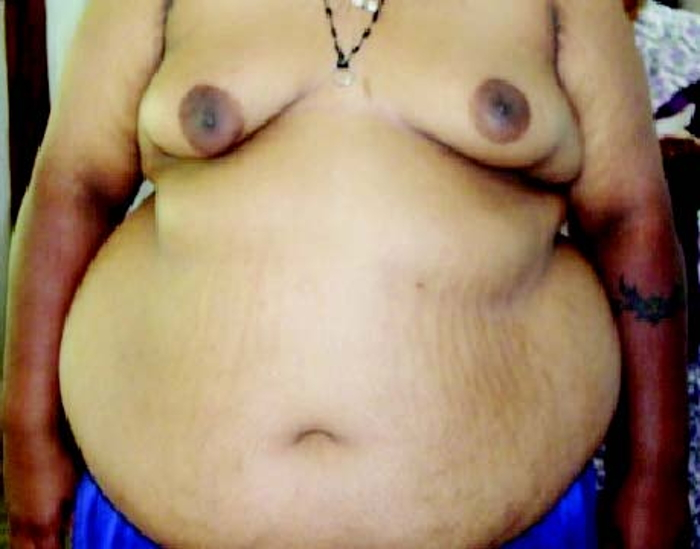
\includegraphics[scale=.6]{images/029.jpg} 
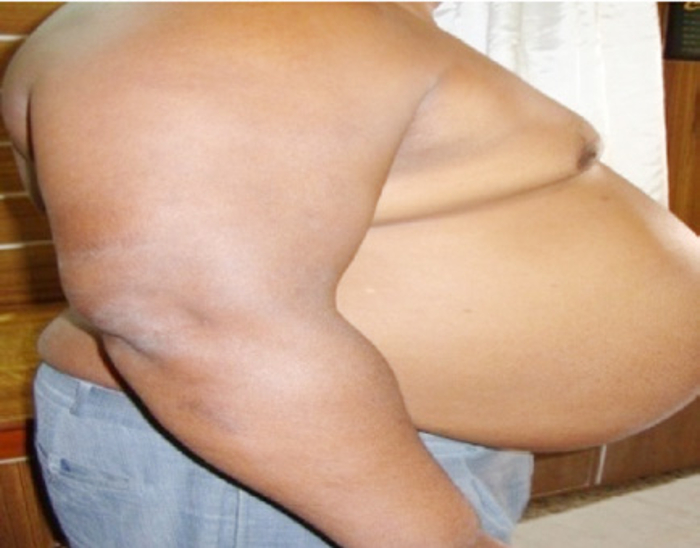
\includegraphics[scale=.6]{images/030.jpg}\\
\textbf{\textit{Pot-belly}}
\end{tabular}
\end{center}

\item Indians face an uphill battle against body fat from infancy itself. Studies done in newborn babies show that Indian babies are born smaller but have a relatively higher body fat content compared to Caucasian babies. \textcolor{red}{\textit{This phenomenon is known as “the thin fat Indian baby”}}.$^{\text{\cite{chap8–key04}}}$ In fact, this pattern persists into childhood, and could be a harbinger of type 2 diabetes in adulthood.$^{\text{\cite{chap8–key05}}}$
\item \textbf{Earlier onset of diabetes in Indians:} Indians tend to develop diabetes about 10 years sooner than Caucasians.
\end{enumerate}

\textbf{Lifestyle changes – the dark side of India’s economic development Junk food}

India is an emerging economic superpower today. Multinational food chains such as Pizza Hut, Starbucks, McDonalds etc. dot the urban landscape now. Eating / hanging–out in these joints is the ‘in–thing’ today for our youth, and is extremely convenient for the working mi\-ddle class. Our young country is eagerly devouring these high–calorie, high–fat ‘junk foods’. This has resulted in an epidemic of obesity in our country.

\noindent\textbf{Sedentary lifestyle}

Another lifestyle factor that is powering the diabetes epidemic is the sedentary lifestyle that the country is getting lulled into.

Not too long ago, agriculture was still the main occupation of our country. It involved hard work that burnt calories and kept people in good health. But slowly the country’s economy has shifted to white–collar (office) jobs due to several factors such as a more educated work force, increased migration to urban areas etc. People are spending more time sitting down than at any other time in human history. Once they go home after work or school, people are at the mercy of the\break latest technology. Adults are glued to their LCD or plasma television, and kids are busy playing video games on their parents cell phones!

Also, people used to walk to work, or bicycle to work up to the 1980s, and early 1990s. Cars were a luxury only a privileged few could afford. But today, with the advent of small cars priced at about 1 lakh rupees, and with increased purchasing capacity, car and two–wheeler ownership has skyrocketed. So has our blood pressure as we spend hours in traffic jams and crawling traffic everyday in Delhi, Mumbai, Bengaluru and other parts of the country.
 
 \clearpage
\noindent\textbf{Stress and sleep disturbance}

\vskip 8pt
Speaking of stress, there is plenty of it in modern day India.\break Software and call center jobs are the face of urban India today. They are powering India’s prosperity and job growth. But they also present certain unusual challenges. Due to the nature of the work, many are forced to work long hours and at odd times. It is not uncommon for some employees to work predominantly during night shifts to acco\-mmodate overseas clients. This destroys our regular sleep–wake cycle, and confuses the body and mind. This results in hormonal imbalances, and increased stress that releases adrenaline. These bodily changes ultimately result in hyperglycemia, which is a natural response of the human body to stress.

The World Health Organization (WHO) and the Indian Council of Medical Research (ICMR) tested these hypotheses in a recent study in India. It was found that diabetic patients were more sedentary and had higher educational qualifications than non–diabetic patients. In this study abdominal obesity and physical inactivity were the main risk factors to develop diabetes.$^{\text{\cite{chap8–key06}}}$

\vskip 8pt
\noindent\textbf{Epidemiologic transition}

\vskip 8pt
This refers to the change in characteristic of the population over time. There have been marked changes in our country, both positive and negative.

Some of the positive changes include – improved nutrition,\break better hygiene, increased access to health care, decreasing deaths from communicable diseases and vaccine preventable diseases. As a consequence people are living longer. For example, in 1947, the ave\-rage life expectancy was 30 years. Today the average Indian lives up to 65 years of age. With increasing age, the total number of Insulin–secreting beta cells in the pancreas decreases, thereby increasing the chances of deve\-loping diabetes.

Due to overall better health status of the country, our population has exploded. In 1947, our population was 37 crores, today it is about 120 crores. This has also contributed to more number of diabetes cases.

\vskip 6pt
\noindent\textbf{Undiagnosed diabetes and prediabetes: the lurking danger!}

\vskip 6pt
\noindent\textbf{Undiagnosed cases}

So far we have discussed only about established (diagnosed) cases of diabetes. But there is something very disturbing under the surface. Based on the available studies, there are more undiagnosed than dia\-gnosed cases of diabetes in our country. In the CURES study done in Chennai, 9.1\% were undiagnosed compared to 6.1\% of diagnosed cases. In the ADEP survey conducted in Kerala the prevalence of undiagnosed diabetes was 10.5\% compared to 9.1\% cases of known diabetes.$^{\text{\cite{chap8–key07}}}$

According to the International Diabetes Federation (IDF) chief Jean Claude Mbanya who spoke at the Diabesity Summit in Mumbai on Nove\-mber 8, 2012, nearly 60\% of diabetic cases in India remain undiagnosed (\textit{Source: The Times of India, November 9, 2012}). These individuals who are undiagnosed remain untreated and are at very high risk for disease complications and premature death.

\vskip 8pt
\noindent\textbf{\textit{Prediabetes\index{Prediabetes}}}

Prediabetes is the precursor of diabetes. It is a wake up call to communicate that a person is on the path to develop diabetes. It also tells that it is not too late to reverse it. It includes both impaired glucose tolerance (IGT) and impaired fasting glucose (IFG).

Based on the National Urban Diabetes Survey (NUDS) conducted in 2000 about 14\% of the population has impaired glucose tolerance, and according to the Chennai Urban Rural Epidemiology Study (CURES) conducted in 2004, about 10.2\% have impaired glucose tolerance. In a country with a population of 120 crores, this translates to about 10 crore people who have imminent risk of diabetes. This stage of prediabetes is a huge opportunity for us to intervene and prevent future diabetes.

\noindent\textbf{How does our country compare to the rest of the world?}

Currently available data clearly indicate a significantly increased disease burden among us Indians compared to any other race in the world. Diabetes rates among Indians are almost two times higher than the rest of the world! The future seems even bleaker for Indians, since diabetes rates are projected to explode among our countrymen. The following graphs illustrate this gloomy scenario.

\noindent\textbf{Impact of this epidemic on India: gazing at the crystal ball}

\begin{figure}[h]
\centering
{\small\textbf{Comparison of prevalence of diabetes among different races in U.S.}}\\
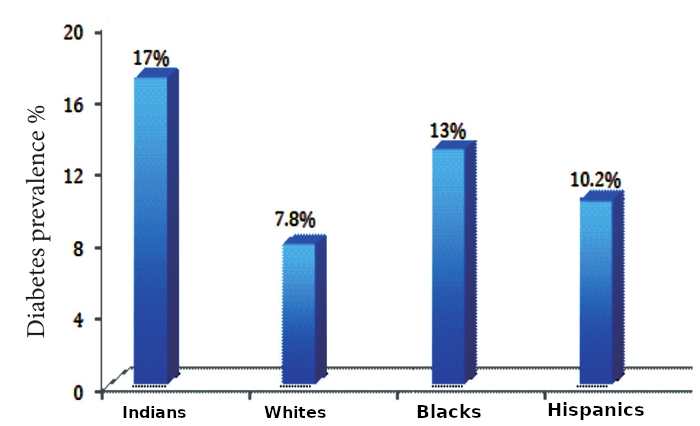
\includegraphics[scale=2.1]{images/031.jpg}
\end{figure}

\noindent\textbf{Differences in prevalence among South Asians and other ethnic groups}

\begin{figure}[h]
\centering
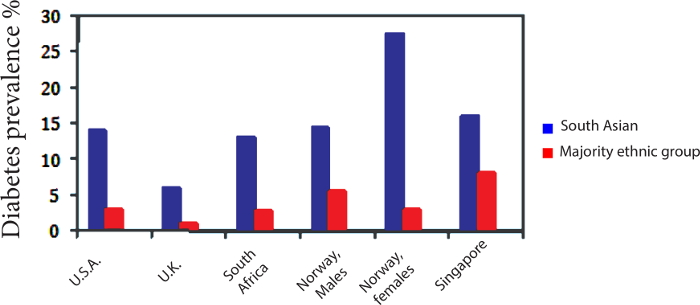
\includegraphics[scale=2.1]{images/032.jpg}
\end{figure}

\clearpage
\begin{center}
Prevalence of diabetes
\end{center}


\begin{figure}[h]
\centering
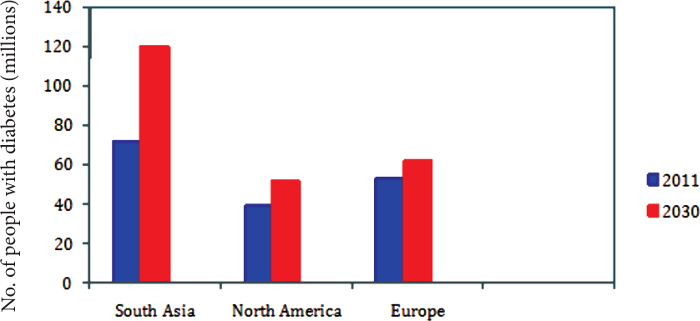
\includegraphics[scale=2.5]{images/033.jpg}
\end{figure}

Type 2 diabetes will be the main driver of the diabetes epidemic, as it accounts for more than 90\% of all diabetes cases. Since Indians are likely to develop this disease 10 years ahead of Westerners, the\break disease will hit individuals in the prime of their lives. Diabetes is very likely to heavily impact our economic prosperity, since a major chunk of individual income will be spent to care for the disease and its\break complications.

\vskip 8pt
\noindent\textbf{How can we prevent this impending national calamity?}

\vskip 8pt
The writing is on the wall when it comes to our country’s future. We must stop this diabetic epidemic dead in its tracks, and it needs to happen today! If not it will severely cripple our economy and society as a whole.

Dr. Vishwanathan Mohan and colleagues at the Madras Diabetes Research Foundation have devised a simple, yet powerful tool to help identify people at risk to develop diabetes. This is called the “Indian Diabetic Risk Score or IDRS”. The following table is a description of this score with all the variables that are assessed and how they are scored.

\begin{center}
\begin{longtable}{|l|c|}
\hline
\multicolumn{1}{|c|}{\textbf{Particulars}} & \textbf{Score}\\
\hline
\textbf{Age} & \\
\hline
\textless 35 years & 0\\
\hline
35-49 years & 20\\
\hline
\textgreater 50 years & 30\\
\hline
\textbf{Waist circumference/abdominal obesity} & \\
\hline
Waist \textless 80 cm (female),\textless 90 cm (male) & 0\\
\hline
Waist \textgreater 80-89 cm (female), \textgreater 90-99 cm (male) & 10\\
\hline
Waist \textgreater 90 cm (female), \textgreater 100 cm (male) & 20\\
\hline
\textbf{Physical activity} & \\
\hline
Vigorous exercise or strenuous (manual) work at & 0\\
home/workplace &\\
\hline
Mild to moderate exercise or mild to moderate & 20\\
physical activity at home/workplace &\\
\hline
No exercise and sedentary activities at home/work & 30\\
\hline
\textbf{Family history} & \\
\hline
No family history & 0\\
\hline
Either parents & 10\\
\hline
Both parents & 20\\
\hline
\multicolumn{2}{@{}l}{\textbf{\textit{Note: This score applies only to type 2 diabetes risk}}}
\end{longtable}
\end{center}

\vskip-.99cm

\noindent Based on this, if the score is:

\begin{enumerate}[•]
\itemsep=0pt
\item \textgreater  60: The risk of having diabetes is VERY HIGH
\item 30–50: The risk of having diabetes is MODERATE
\item \textless  30: The risk of having diabetes is VERY LOW.
\end{enumerate}

\noindent\textbf{In summary:}

Calculating IDRS should not take more than two minutes. A person’s age, family history of diabetes, exercise patterns, and waist\break circumference, are used to calculate a score to predict the risk of that person going on to develop diabetes in future. Studies show that this scoring system is accurate in its predictions. It can serve as a valuable tool that can be used in any corner of India (or world) to identify high–risk groups. These high–risk groups can then be targeted with lifestyle interventions such as diet and physical activity, which can help prevent and/or delay diabetes. This is one of the many simple measures we can adopt to protect our country and citizens from diabetes.


\begin{thebibliography}{99}
\bibitem{chap8–key01} McDermott R, Rowley KG, Lee AJ, Knight S, O’Dea K. Increase in prevalence of obesity and diabetes and decrease in plasma chole\-sterol in a central Australian aboriginal community. Med J Aust. 2000; 172 (10): 480–4.
 \bibitem{chap8–key02} Henry CJ, Lightowler HJ, Newens K, Sudha V, et al. Glycaemic\break index of common foods tested in the UK and India. Br J Nutr. 2008; 99 (4): 840–5.
 \bibitem{chap8–key03} Ramachandran A, Snehalatha C, Vishwanathan V, Vishwanathan M, \&Haffner SM. Risk of noninsulin dependent diabetes mellitus conferred by obesity and central adiposity in different ethnic groups: A comparative analysis between Asian Indians, Mexican Americans and Whites. Diabetes Res ClinPract. 1997; 36 (2): 121–5.
 \bibitem{chap8–key04} Yajnik CS, Fall CH, Coyaji KJ, Hirve SS, et al. Neonatal anthropo\-metry: The thin–fat Indian baby. The Pune Maternal Nutrition Study. Int J ObesRelatMetabDisord. 2003; 27 (2): 173–80.
 \bibitem{chap8–key05} Krishnaveni GV, Hill JC, Veena SR, Leary SD, et al. Truncal adiposity is present at birth and in early childhood in South Indian children. Indian Pediatr. 2005; 42 (6): 527–38.
 \bibitem{chap8–key06} Mohan V, Mathur P, Deepa R, Deepa M, et al. Urban rural differe\-nces in prevalence of self–reported diabetes in India– the WHO–ICMR Indian NCD risk factor surveillance. Diabetes Res ClinPract. 2008; 80 (1): 159–68.
 \bibitem{chap8–key07} Menon VU, Kumar KV, Gilchrist A, Sugathan TN, et al. Prevalence of known and undetected diabetes and associated risk fa\-ctors in central Kerala–ADEPS. Diabetes Res ClinPract. 2006; 74 (3):\break 289–94.
 \bibitem{chap8–key08} Misra R, Patel T, Kotha P, Raji A, et al. Prevalence of diabetes, metabolic syndrome, and cardiovascular risk factors in US Asian Indians: results from a national study. J Diabetes Complications. 2010; 24 (3): 145–53.
 \bibitem{chap8–key09} Gujral UP, Pradeepa R, Weber MB, Narayan KM, \& Mohan V. Type 2 diabetes in South Asians: similarities and differences with White Caucasian and other populations. Ann N Y Acad Sci. 2013; 1281: 51–63.
 \end{thebibliography}


\chapter{Diabetes – Global Picture}\label{chap9}

Today diabetes is a global problem. No country or region is safe from this growing epidemic.

As of 2017, the global prevalence of diabetes is 8.8\% or 425\break million adults. Majority of these diabetics (79\%) live in developing countries. Diabetes prevalence numbers are largely determined by\break people with type 2 diabetes who comprise about 90\% of all diabetics. There are several reasons for the growing diabetes epidemic globally, such as the overall increase in prevalence of diabetes, increase in population growth, increasing lifespan of humans, and the burgeoning\break obesity epidemic.

If current trends persist, it is expected that there will be there will be additional 200 million diabetic adults by 2045, with most of these new cases occurring in the developing countries.

\vskip 9pt

\textcolor{darkorange}{\textbf{Top 5 Countries with most adult (20-79 years) diabetics in\break 2017 \& 2045}$^{\text{\cite{chap9–key01}}}$}

{
\begin{table}
\centering
\begin{tabular}{|c|c|c|c|c|c|}
\hline
\multicolumn{3}{|c|}{{\cellcolor{lightblue}\large\textbf{2017}}} & \multicolumn{3}{c|}{{\cellcolor{yellow}\large\textbf{2045}}}\\
\hline
 & \multirow{2}{1.4cm}{\textbf{Country}} & \textbf{Number of} &  & \multirow{2}{1.4cm}{\textbf{Country}} & \textbf{Number of}\\
 &  & \textbf{diabetics} &  &  & \textbf{diabetics}\\
 \hline
1 & China & 114 million & 1 & India & 134 million\\
 \hline
2 & India & 72 million & 2 & China & 120 million\\
 \hline
3 & USA & 30 million & 3 & USA & 36 million\\
 \hline
4 & Brazil & 12.5 million & 4 & Mexico & 22 million\\
 \hline
5 & Mexico & 12 million & 5 & Brazil & 20 million\\
 \hline
\end{tabular}
\end{table}
}\relax

\clearpage

\begin{figure}[h]
\centering
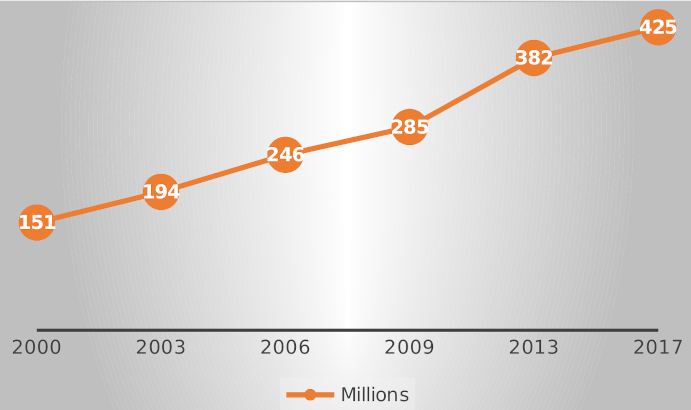
\includegraphics[scale=2.3]{images/034.jpg}\\
\textcolor{darkorange}{\textbf{Total number of adults (20-79 years) with diabetes globally$^{\text{\cite{chap9–key01}}}$}}
\vskip -.2cm
\end{figure}

Global diabetes prevalence has increased both among males and\break females. The prevalence of diabetes in males was 4.3\% in 1980, but\break doubled to 9\% by 2014. In females, it was 5\% in 1980 and increased to 7.9\% by 2014.

Diabetes remains a mostly urban disease, and is projected to\break remain so in the future, likely due to continued migration of humans from rural to urban areas. It is well known that sedentary lifestyle and high calorie intake, which are part of parcel of urban life are significant risk factors to develop diabetes.

These figures are likely to be a significant underestimate of the\break actual burden of diabetes, since 30-80\% of diabetes remain undia\-gno\-sed. Low income countries without adequate resources to allocate for early diagnosis of diabetes have a higher prevalence (76.5\%) of undia\-gnosed diabetes.

The International Diabetes Federation (IDF) estimates one death every seven seconds from diabetes or its complications, with 50\% of those deaths (4 million total diabetes related deaths per year)\break occurring under the age of 60 years$^{\text{\cite{chap9–key01}}}$.

\clearpage

{
\begin{table}[H]
\centering
\caption*{\textcolor{darkorange}{\textbf{Top 5 Countries with undiagnosed diabetics$^{\text{\cite{chap9–key01}}}$}}}
\vskip -.5cm
\begin{longtable}{|c|c|c|c|}
 \hline
 &  & \textbf{Number of} & \multirow{2}{1.8cm}{\textbf{Proportion}}\\
 & \textbf{Country} & \textbf{undiagnosed} & \multirow{2}{2.1cm}{\textbf{undiagnosed}}\\
 &  & \textbf{diabetics} & \\
\hline
1  & China & 61.3 million & 53.6\%\\
 \hline
2 & India & 42.2 million & 57.9\%\\
 \hline
3 & USA & 11.5 million & 38.2\%\\
 \hline
4 & Indonesia & 7.6 million & 73.7\%\\
 \hline
5 & Brazil & 5.7 million & 46\%\\
 \hline
\end{longtable}
\end{table}
}\relax

\vskip -.5cm

\noindent\textbf{Global prevalence of impaired glucose tolerance (IGT)}

In addition to overt diabetes, the IDF estimates another 352.1\break million people worldwide to have a precursor stage of diabetes, called impaired glucose tolerance (IGT), a figure which is anticipated to rise to 587 million in 2045. Majority of these cases are from the developing parts of the world (72.3\%), and are below the age of 50 years (49\%)1.

\textcolor{darkorange}{\textbf{Top 5 Countries with impaired glucose tolerance (IGT)$^{\text{\cite{chap9–key01}}}$}}


{
\begin{center}
\begin{tabular}{|c|l|c|}
\hline
 & \multirow{2}{1.6cm}{\textbf{Country}} & \textbf{Population}\\
 &  & \textbf{with IGT}\\
 \hline
1 & China & 48.6 million\\
 \hline
2 & USA & 36.8 million\\
 \hline
3 & Indonesia & 27.7 million\\
 \hline
4 & India & 24 million\\
 \hline
5 & Brazil & 14.6 million\\
 \hline
\end{tabular}
\end{center}
}\relax

This is a population that is at cross roads. At the stage of IGT, lifestyle modifications such as diet and exercise may delay or prevent the onset of diabetes and its complications. However, if nothing is done, they are likely to go on to develop diabetes.

According to recent studies, about five percent of the total diabetes population represents Monogenic forms of diabetes, such as various subtypes of MODY (Maturity onset Diabetes of the Young) and other rare genetic conditions, another five percent comprises sub–forms of immune–Mediated type 1 diabetes with a pronounced, insulin deficit in the long run.$^{\text{\cite{chap9–key01}}}$

Consequent to enormous therapeutic progress in the last thirty years, many people affected with type 1 diabetes today are able to live for almost a normal life span, although the disease usually starts at a young age, i.e. in children and adolescents.

\begin{thebibliography}{99}
\bibitem{chap9–key01} International Diabetes Federation. IDF Diabetes Atlas, 8th edn. Brussels, Belgium: International Diabetes Federation, 2017. http://www.diabetesatlas.org; last accessed on January 23, 2019.
\end{thebibliography}




